% MAREA manuscript — working draft.
% Build: bash build.sh   (MiKTeX; elsarticle, numbered citations, elsarticle-num)
% Every number here traces to a notebook, a script or results/*.json; every
% literature claim to literature_quotes.md (verbatim passages with pages).
% Hard limit set by the author (2026-09-23): 12 pages in all, title,
% abstract, references and acknowledgements included, with many figures.
% Journal two-column layout (final,5p): the same text in the 12pt preprint
% layout runs to more than twice the pages.
\documentclass[final,5p,times,number]{elsarticle}

\usepackage{amsmath,amssymb}
\usepackage{graphicx}
\usepackage{booktabs}
\usepackage[hidelinks]{hyperref}
\usepackage{etoolbox}
% reference list in footnotesize, as the journal sets it (page limit)
\AtBeginEnvironment{thebibliography}{\footnotesize}
\makeatletter\@ifundefined{bibsep}{}{\setlength{\bibsep}{0pt plus 0.3ex}}\makeatother
% the three results figures after the bibliography may share one page
\setcounter{topnumber}{3}\setcounter{bottomnumber}{2}\setcounter{totalnumber}{4}
\renewcommand{\topfraction}{0.95}\renewcommand{\bottomfraction}{0.95}
\renewcommand{\textfraction}{0.05}\renewcommand{\floatpagefraction}{0.6}
\graphicspath{{figures/}{../figures/}{../figures/tide_comparison/}{../figures/onepixel/}}

% target journal is a placeholder until decided
\journal{Remote Sensing of Environment}

\begin{document}

\begin{frontmatter}

\title{Timing the tide from space: intertidal topography from Sentinel-2
  with the estuarine tide measured from the imagery itself}
% alternative titles kept in draft.md

% TODO: confirm names, order and affiliations
\author[a]{Jorge Alias \'Alvarez\corref{cor1}}
\author[b]{[Supervisor 1]}
\author[c]{[Supervisor 2]}
\cortext[cor1]{Corresponding author}
\affiliation[a]{organization={[Affiliation 1]}, city={Oviedo}, country={Spain}}
\affiliation[b]{organization={[Affiliation 2]}, country={Spain}}
\affiliation[c]{organization={[Affiliation 3]}, country={Spain}}

\begin{abstract}
Satellite archives allow the topography of tidal flats, among the most
extensive and most threatened coastal ecosystems, to be mapped by
reading for every pixel the water level at which it floods. Every
published implementation assigns each scene one water level from a tide
model or gauge at one point. Inside an estuary that level is wrong: the
tide arrives later and deformed the farther it travels up the channel,
so the error grows inland and is systematic. MAREA measures this
interior lag from the imagery itself. Each intertidal pixel is a binary
tide gauge; for each 3-km band of along-channel distance the lag that
best explains its ten-year wet/dry record maximises a profiled
Bernoulli likelihood anchored at the mouth, the lags monotone by
construction, each with a bootstrap interval. A binary archive measures
the phase of the interior tide but not its amplitude or datum; only the
phase is corrected. On four European estuaries with gauge pairs, MAREA
measured lags of 63 and 129~min at the inner gauges of the Ems-Dollard
and the Wadden Sea, where the gauges show 51 and 88, applied 7~min in
the Westerschelde and none in the R\'ia de Ferrol, and cut the
water-level error at the inner gauge by 42 and 46\,\% in the two large
estuaries. Against the official Dutch bathymetry its maps reach 0.33 to
0.44~m RMSE with slopes of 0.65 to 0.81, against 0.48 to 0.78~m for the
published logistic alternative; against an RTK-GNSS survey in the
R\'ia de Villaviciosa (Spain) the estimator reaches 0.19~m RMSE with a
slope of 0.72, against 0.27~m and 0.39 for the alternative. The method
needs no instrument inside the estuary; code, notebooks and negative
results are released.
\end{abstract}

\begin{keyword}
intertidal topography \sep tidal flats \sep Sentinel-2 \sep tidal
propagation \sep estuaries \sep waterline method \sep tide models \sep
profile likelihood \sep digital elevation model
\end{keyword}

\end{frontmatter}

% Highlights (Elsevier asks for them as a separate file at submission; the
% text is kept in draft.md, not in the manuscript body).

\section{Introduction}

Tidal flats (Fig.~\ref{fig:flats}) are among the most extensive and
least mapped coastal ecosystems: the first global inventory found at
least 127\,921~km$^2$ and a 16\,\% loss between 1984 and 2016
\cite{murray2019}. They are productive and buffer the coast
\cite{sagar2017}, and their elevation governs flooding, habitat and
surge exposure, yet coastal topography is coarse, outdated or absent
over much of the world \cite{almar2021} because surveying a mudflat is
slow, expensive and often dangerous \cite{bell2016,sagar2017}. Global
surface-water products ignore the tidal stage of each image
\cite{pekel2016,fitton2021}, the orbit samples the tide unevenly
\cite{eleveld2014} and clear low-tide scenes are scarce: four usable
Sentinel-2 images a year at Santander Bay, on the coast studied here
\cite{davies2024}.

The archive offers a way round the survey: the tide scans the relief,
and a dated image series is a series of yes/no questions about every
pixel's elevation. Waterline methods \cite{mason1995,ryu2008} tag each
scene's land--water contour with the water level at acquisition and
interpolate between contours, with sub-pixel refinements
\cite{bishoptaylor2019waterline,vos2019}, and have produced continental
models \cite{sagar2017,bishoptaylor2019ecss,fitton2021}. Per-pixel
methods fit a logistic curve to each pixel's response against water
level, its midpoint the elevation, from X-band SAR \cite{catalao2017},
Sentinel-2 near-infrared reflectance \cite{bue2020,granadeiro2021} or
the water/land class \cite{chen2025}, or cross-correlate radar series with
the wet/dry sequence of each candidate elevation \cite{bell2016}. These
are the quantal-response ogives of Gaddum~\cite{gaddum1933} and
Bliss~\cite{bliss1934}, the probit and logit of Finney and Berkson
\cite{finney1947,berkson1944}: a shoreline pixel is a mixture whose
index tracks its water fraction
\cite{rover2010,feyisa2014,bishoptaylor2019waterline}, the cumulative
distribution of its internal relief, with the elevation at its 50\,\%
point.

\begin{figure}[t]
\centering
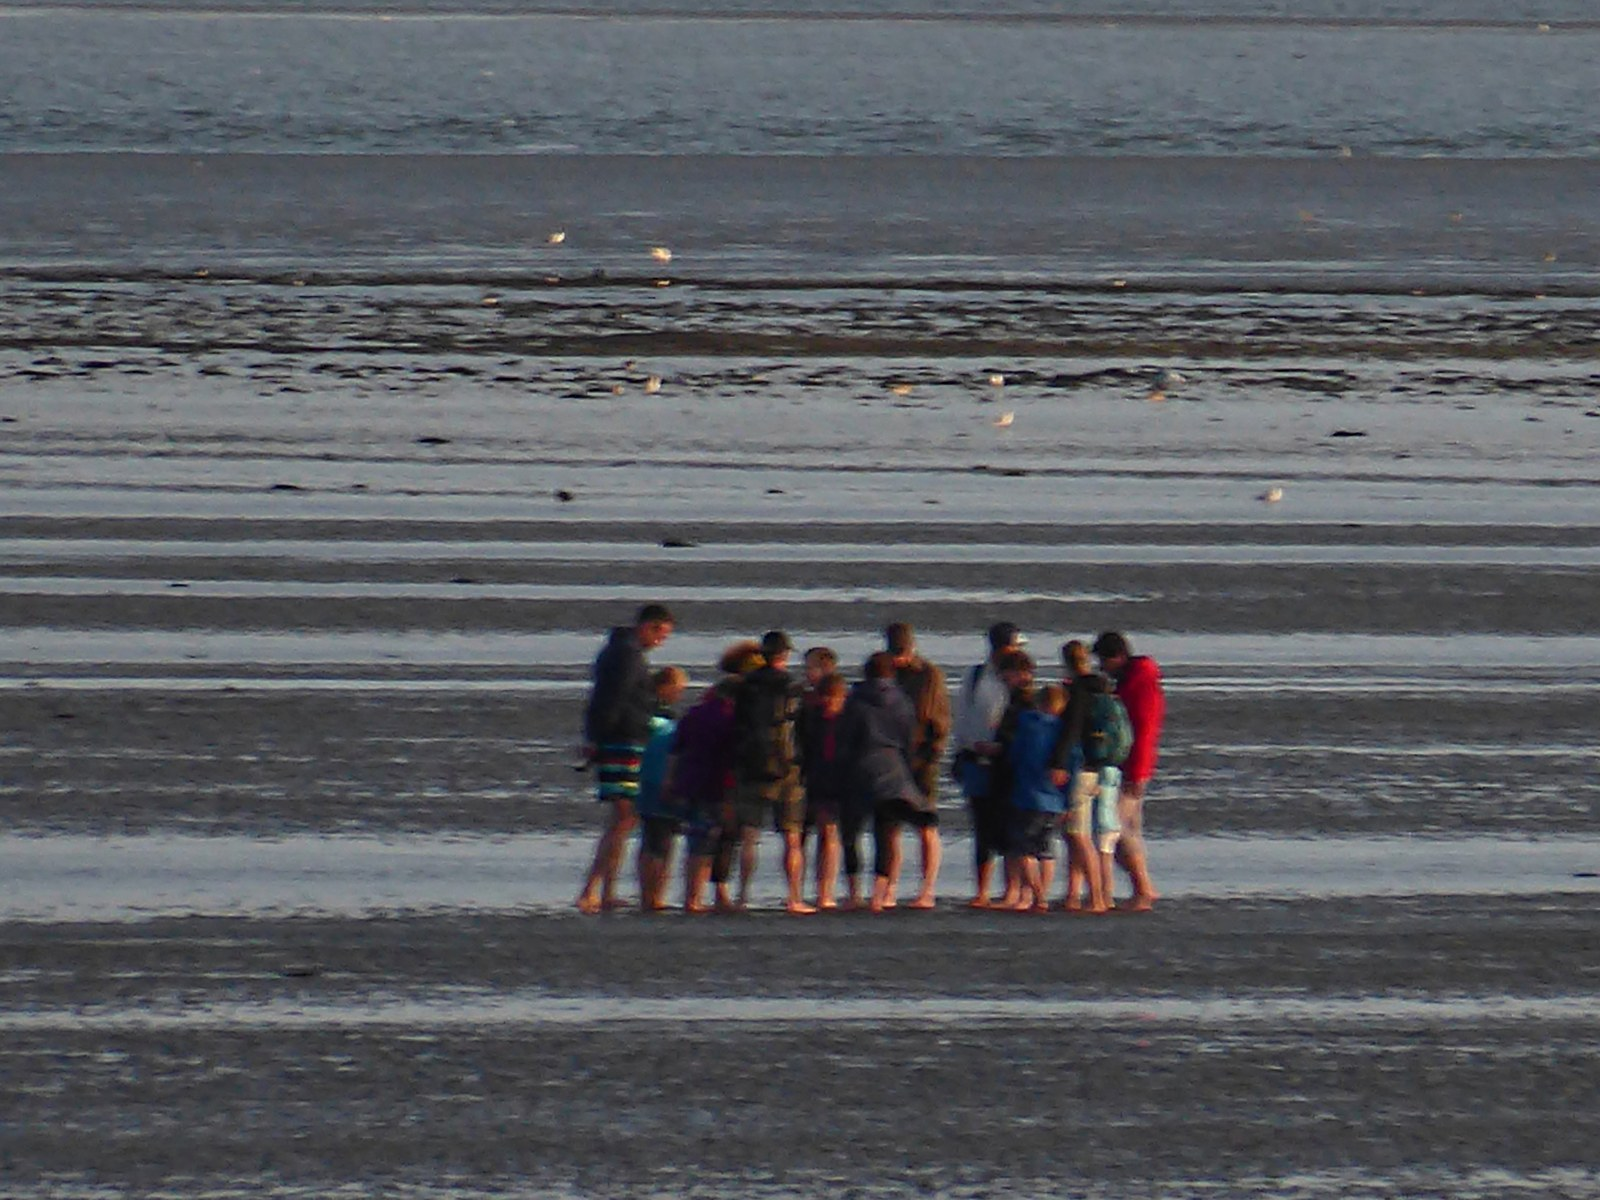
\includegraphics[width=0.49\columnwidth]{figures/fig1_wadden_walk_cc0.jpg}\hfill
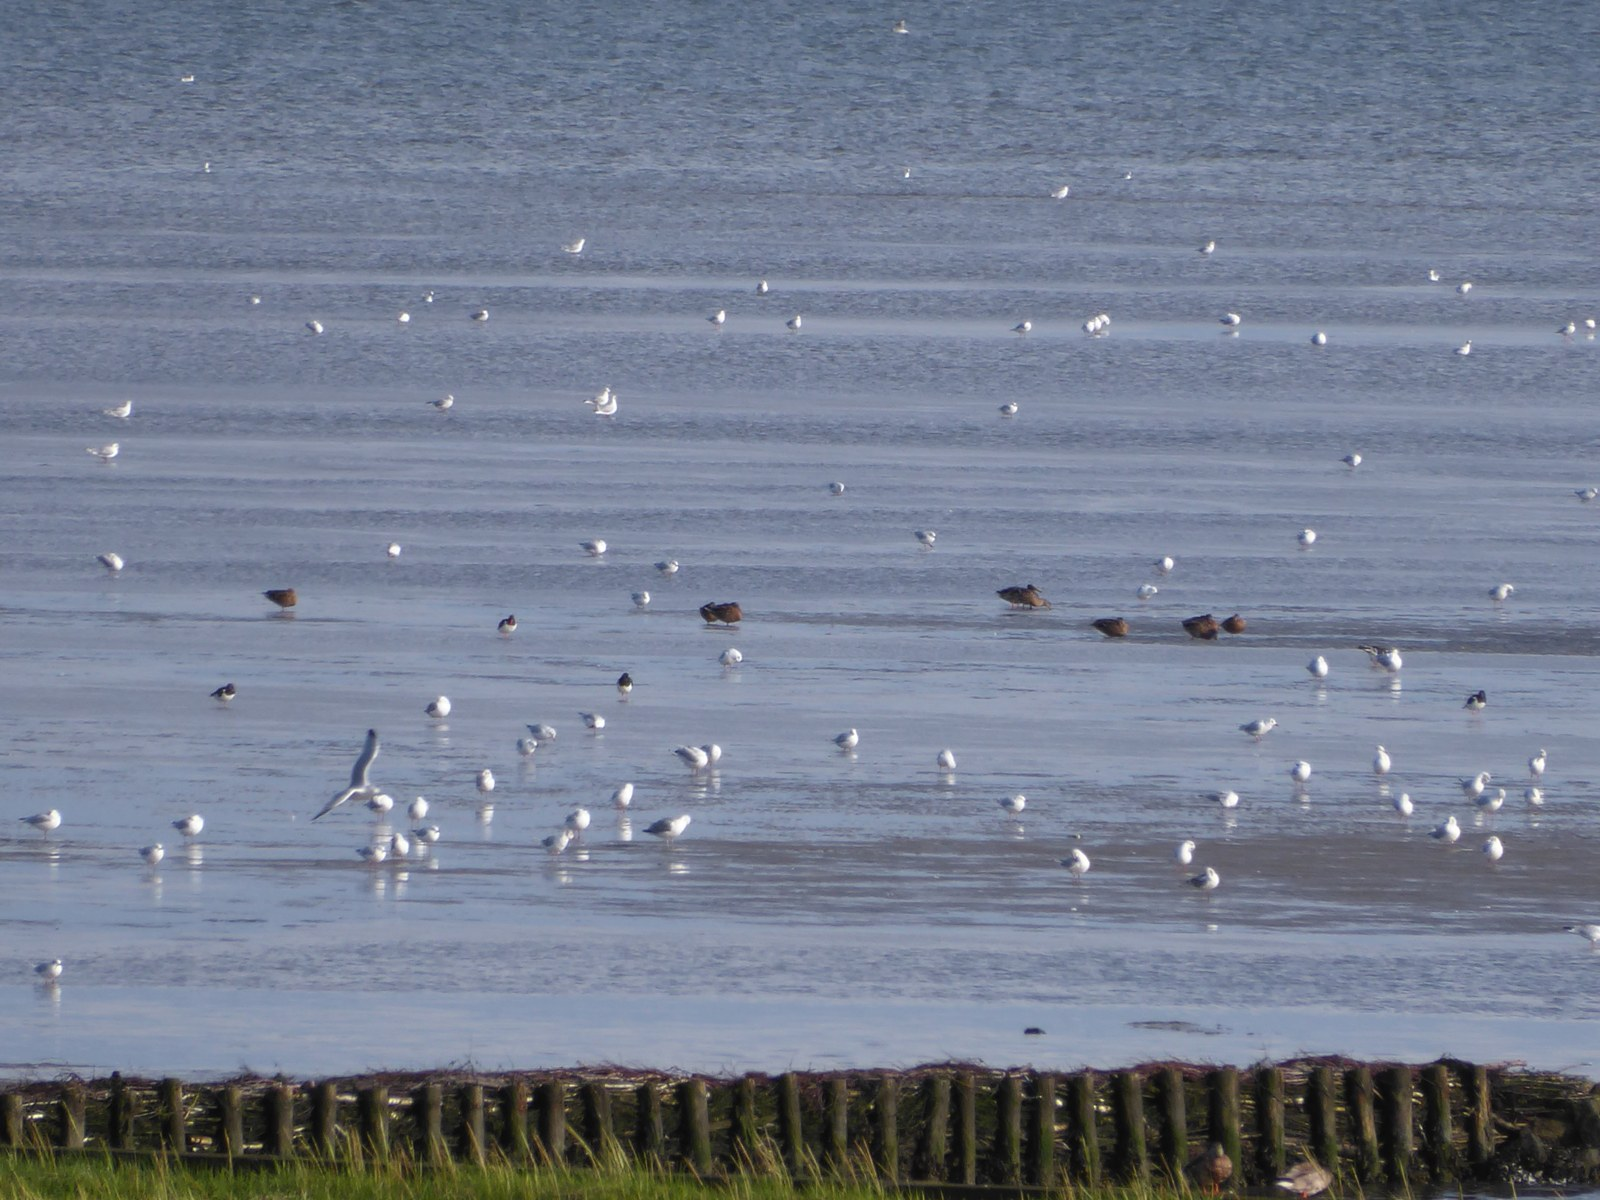
\includegraphics[width=0.49\columnwidth]{figures/fig1_wadden_groyne_cc0.jpg}
\caption{Tidal flats at low water (German Wadden Sea, Wangerooge, August
2019). Left, a guided walk across flats that the next high water will
cover; right, the edge of the flat at a groyne, with gulls and waders on
the exposed mud. Photographs by Rhetos, Wikimedia Commons, CC0 1.0.}
\label{fig:flats}
\end{figure}

All share one input: the water level of each scene, from a tide model or
gauge at one point, applied to the whole scene or cell
\cite{sagar2017,bishoptaylor2019ecss,bue2020,fitton2021,granadeiro2021,chen2025}.
The caveat is on record: a single instantaneous level ``is no doubt a
simplification of reality'' \cite{sagar2017}; accuracy falls with
distance from the modelling point, with lags in estuaries
\cite{bishoptaylor2019ecss}; part of a $-0.51$~m bias on the Tagus
comes from ``different tide height values for the same image
acquisition time'' \cite{bue2020}; phase differences exceed one hour
within one Sentinel-2 scene \cite{granadeiro2021}; a mean absolute
error fell from 0.64 to 0.46~m with a closer gauge \cite{chen2025}; and
a shore-based radar measured a bias of 0.12~m within 0.75~km of the
gauge and about 0.5~m beyond \cite{bell2016}. Every reported survey
accuracy, from $\pm 0.39$~m \cite{bishoptaylor2019ecss} to 0.57~m
\cite{sagar2017}, carries this error.

Global tide models cannot remove it (Fig.~\ref{fig:schematic}): they
stop at the coast. FES2014
\cite{lyard2021}, EOT20 \cite{hartdavis2021} and TPXO \cite{egbert2002}
reach about 2~cm in the open ocean but diverge near the coast
\cite{hartdavis2021}. EOT20 discards altimetry within 3 to 7~km of the
coast and holds no observation inside an estuary; FES2014 resolves at
best 1.5~km in estuaries, sees no water shallower than 10~m,
down-weights coastal gauges and calls estuaries and deltas an open
problem \cite{lyard2021}. Inter-model differences exceed 30~cm near
coasts, with metre-level errors at individual gauges \cite{wang2025},
and the best regional ensemble still leaves 0.29 to 0.36~m at sheltered
inlets, with ``visible sharp elevation discontinuities'' traced to a
phase error \cite{bishoptaylor2026}. Inside an estuary the tide arrives
later the farther it travels, amplified by convergence, damped by
friction and distorted in shallow water
\cite{friedrichs1994,savenije2005}, so a level read at the mouth is
wrong inland by an amount that grows with distance and repeats in every
scene.

Two studies read tidal information from the imagery itself. Granadeiro
et al.~\cite{granadeiro2021} fit separate logistic curves to rising and
ebbing scenes and take the lag that reconciles the two elevations,
giving cotidal lines over the Bijag\'os archipelago within 6.6~min of
the official values at five stations; it returns one lag per location,
needs a reference site with a known tide and was tested on an open
archipelago, not an estuary. Bishop-Taylor et
al.~\cite{bishoptaylor2026} rank ten global tide models by the
correlation of each pixel's NDWI with the modelled tide, which reads
phase but could rank a model highly ``even if it greatly misrepresented
tidal amplitude'', and leave estuarine amplification and damping
uncovered. Neither estimates the interior lag with a statistical model
of the pixel, states what a wet/dry archive can identify, or tests a
measured lag against sampling noise.

This paper does those three things. MAREA treats every intertidal pixel
as a binary tide gauge, a Rasch-type model with scenes as persons and
pixels as items \cite{rasch1960,engelhard2021}, and measures the phase
lag of the estuarine tide from the Sentinel-2 archive alone: per 3-km
band of along-channel distance, the lag that best explains the ten-year
wet/dry record maximises a profiled Bernoulli likelihood, each pixel's
elevation and width refitted under every candidate lag
\cite{golub1973,kaufman1975}, anchored at the mouth to a boundary that
never includes the judge gauge. Binary data identify phase but not gain
or datum; the lags are monotone inland by construction and each carries
a bootstrap interval. Validation uses four European estuaries with
gauge pairs, the official Rijkswaterstaat bathymetry at the Dutch
sites, and the R\'ia de Villaviciosa (Spain) with an RTK-GNSS survey,
against the method of Granadeiro et al.~\cite{granadeiro2021}
reimplemented on the same pixels.

\begin{figure}[t]
\centering
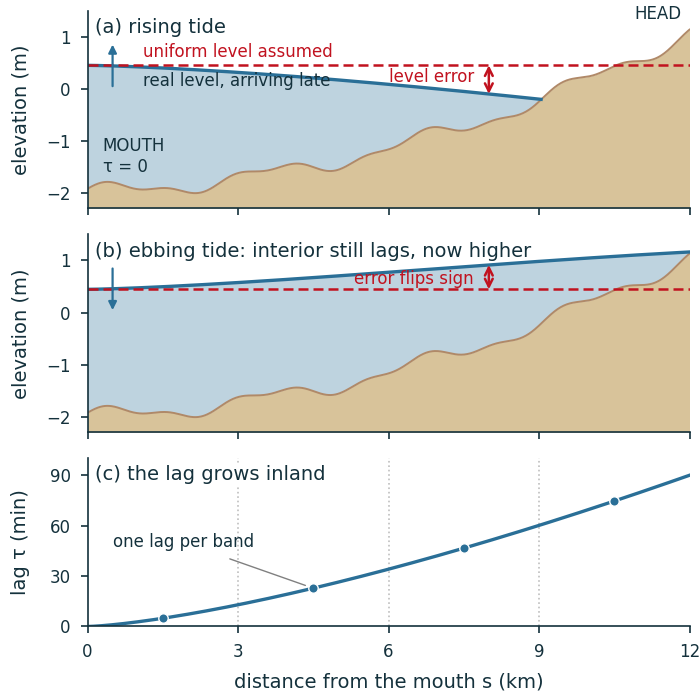
\includegraphics[width=\columnwidth]{fig_schematic.png}
\caption{The error the method measures. (a) On a rising tide the water
surface inside an estuary slopes down inland because the tide arrives
late; the single level every published method reads at the mouth
(dashed) is wrong by an amount that grows with distance. (b) On the ebb
the interior still lags, so the sign of the error flips with the limb.
(c) The lag $\tau$ grows with the distance $s$ from the mouth; MAREA
measures one lag per 3-km band of $s$.}
\label{fig:schematic}
\end{figure}

\section{Methods}\label{sec:methods}

\subsection{Study sites and data}\label{sec:sites}

\subsubsection{Sites}

The method was developed on the R\'ia de Villaviciosa and its interior
clock tested on four other estuaries (Fig.~\ref{fig:sites},
Table~\ref{tab:sites}). Villaviciosa is a 7~km drowned valley on the
Cantabrian coast of Spain, one channel with mudflats on both banks; its
ten-year archive at 10~m (1\,379 scenes) was the test bed of every stage
and holds the only field survey, an RTK-GNSS transect. The r\'ia has no
tide gauge, so its boundary is the ocean model alone, and the measured
lag on the transect is a few minutes: Villaviciosa validates the
estimator more than the clock.

\begin{figure*}[t]
\centering
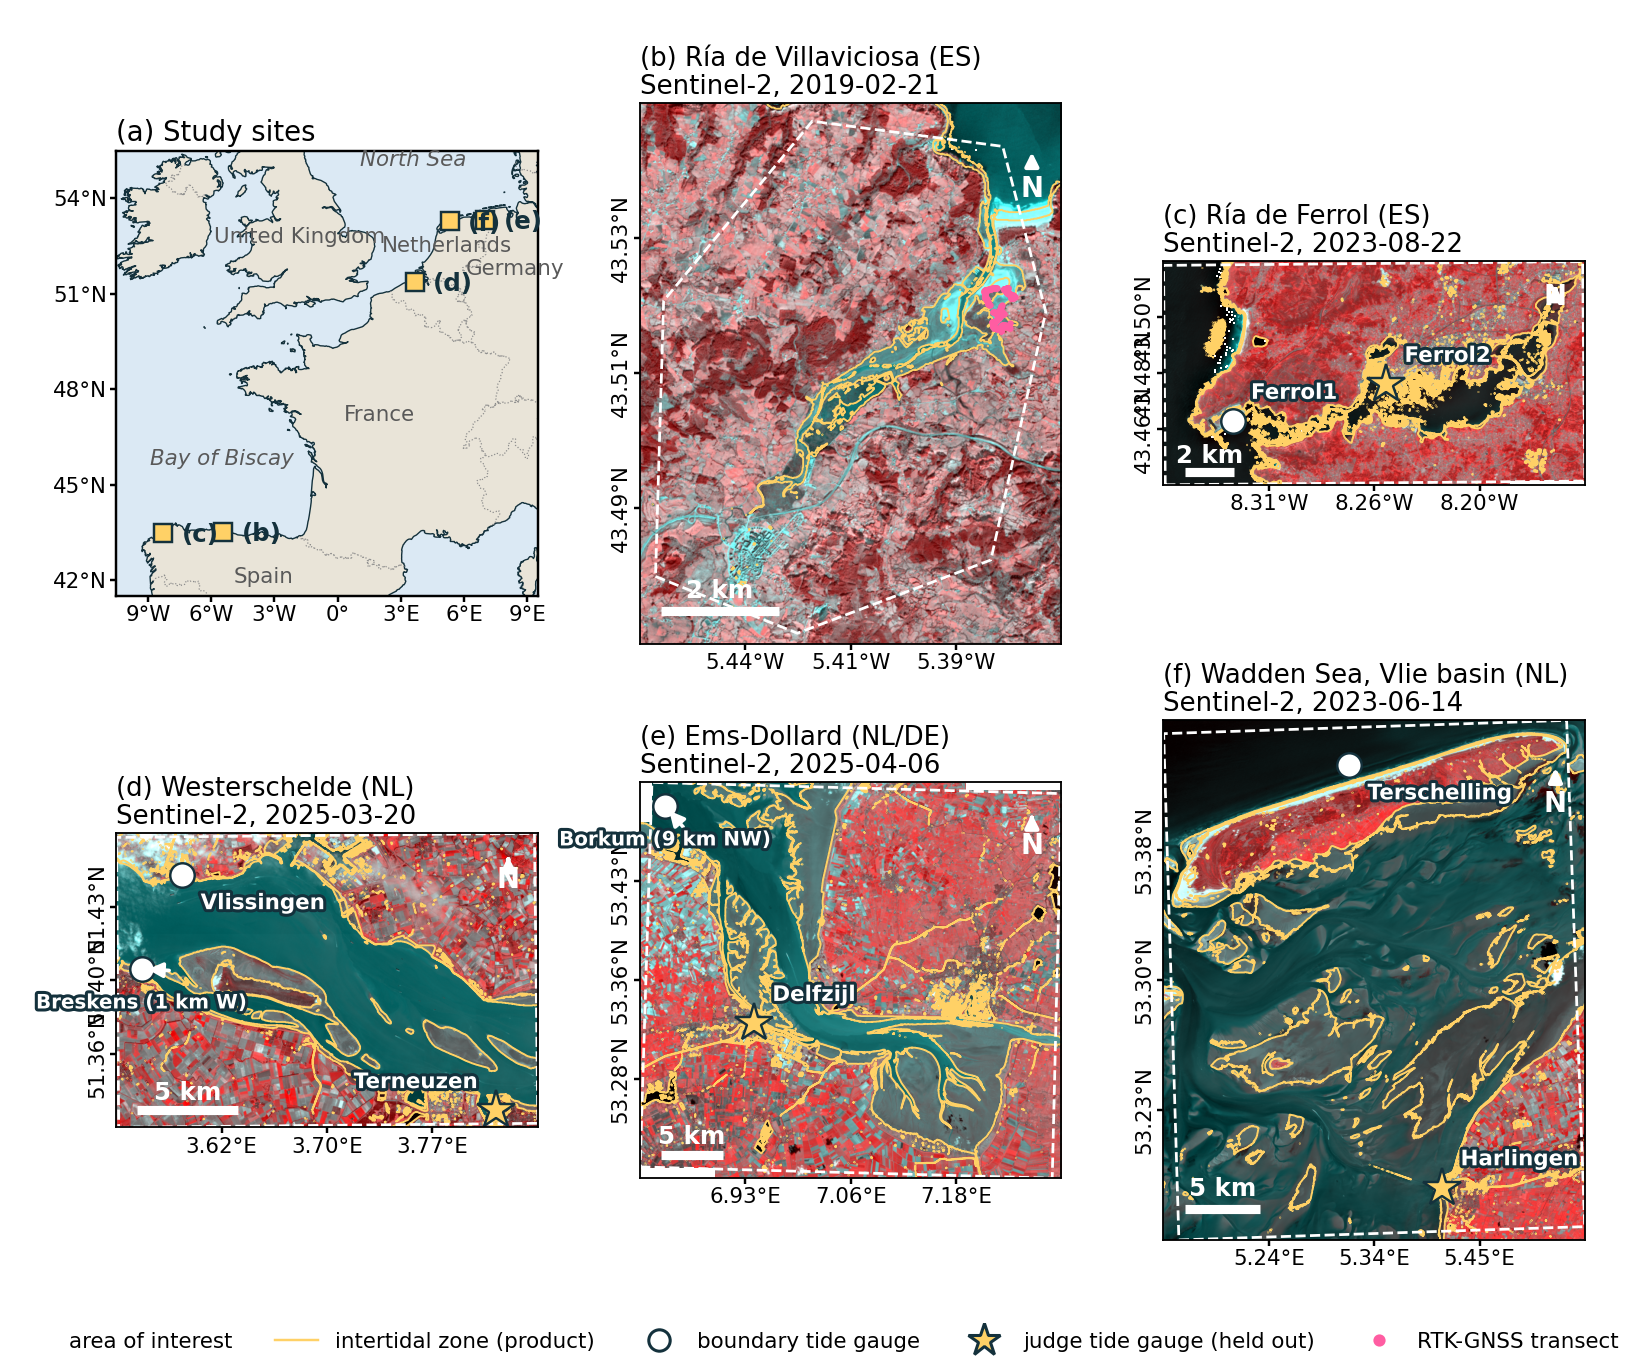
\includegraphics[width=0.60\textwidth]{figures/fig_sites.png}
\caption{Study sites. (a) The five sites on the Atlantic and North Sea
coasts of Europe (Natural Earth coastline). (b)--(f) Each site on a clear
low-water Sentinel-2 scene from its datacube, as a false-colour composite
(near-infrared, green, green: water dark, exposed sediment grey,
vegetation red). Dashed line, area of interest; yellow outline, intertidal
zone retained by the product; circles, tide gauges feeding the boundary;
star, gauge held out as judge; a gauge outside the frame is marked at the
nearest edge with its distance. In (b) the magenta points are the
development subset of the RTK-GNSS survey. Scene dates are in the panel
titles.}
\label{fig:sites}
\end{figure*}

The four test sites were chosen by one criterion: two tide gauges on
one tidal axis, one at the mouth to feed the boundary and one inside to
judge, never entering any fit. The R\'ia de Ferrol (Galicia), short and
deep, is the negative control: the tide should arrive almost unchanged.
The Westerschelde is the funnel mouth of the Scheldt between Vlissingen
and Terneuzen; the Ems-Dollard (Netherlands and Germany) is a 35~km
estuary whose inner basin, the Dollard, is a mudflat bay behind a
constricted channel; the Wadden site is the Vlie basin between
Terschelling and Harlingen.

\begin{table*}[t]
\centering
\caption{Study sites. Scenes are all Sentinel-2 L2A acquisitions in the
period at the stated resolution, before cloud screening; intertidal
pixels have water frequency between 0.10 and 0.90 and at least 30 clear
observations; the judge's distance is the geodesic distance through the
water from the sea edge of the site.}
\label{tab:sites}
\footnotesize
\setlength{\tabcolsep}{4pt}
\resizebox{\textwidth}{!}{%
\begin{tabular}{@{}lrrrlll@{}}
\toprule
site & res. & period & scenes & intertidal px & boundary gauges & judge (km) \\
\midrule
R\'ia de Villaviciosa (ES)$^{a}$ & 10 m & 2016--25 & 1\,379 & --- & none (EOT20 only) & none \\
R\'ia de Ferrol (ES) & 10 m & 2023--25 & 461 & 103\,759 & Ferrol1 & Ferrol2 (10.1) \\
Westerschelde (NL)$^{b}$ & 20 m & 2023--25 & 464 & 73\,764 & Vlissingen, Breskens & Terneuzen (21.9) \\
Ems-Dollard (NL/DE)$^{b}$ & 20 m & 2023--25 & 462 & 477\,745 & Borkum & Delfzijl (24.4) \\
Wadden, Vlie basin (NL)$^{b}$ & 20 m & 2023--25 & 462 & 367\,076 & Terschelling & Harlingen (18.3) \\
\bottomrule
\multicolumn{7}{@{}l@{}}{$^{a}$ elevation truth: RTK-GNSS survey. $^{b}$ elevation truth: Rijkswaterstaat Vaklodingen.}
\end{tabular}}
\end{table*}

Beyond the five sites, the pipeline ran unattended on 130 cells of
10~km along the north coast of Spain, from the R\'ia de Ribadeo to the
Bidasoa (Fig.~\ref{fig:census}), 286~km$^2$ of intertidal ground with a
median of 461 scenes per cell; under the detection rule then in force,
108 cells applied an interior lag and 21 kept the uniform level, with a
median largest lag of 24~min per cell. The census is released with the
code; its cells are not validated here.

\begin{figure*}[t]
\centering
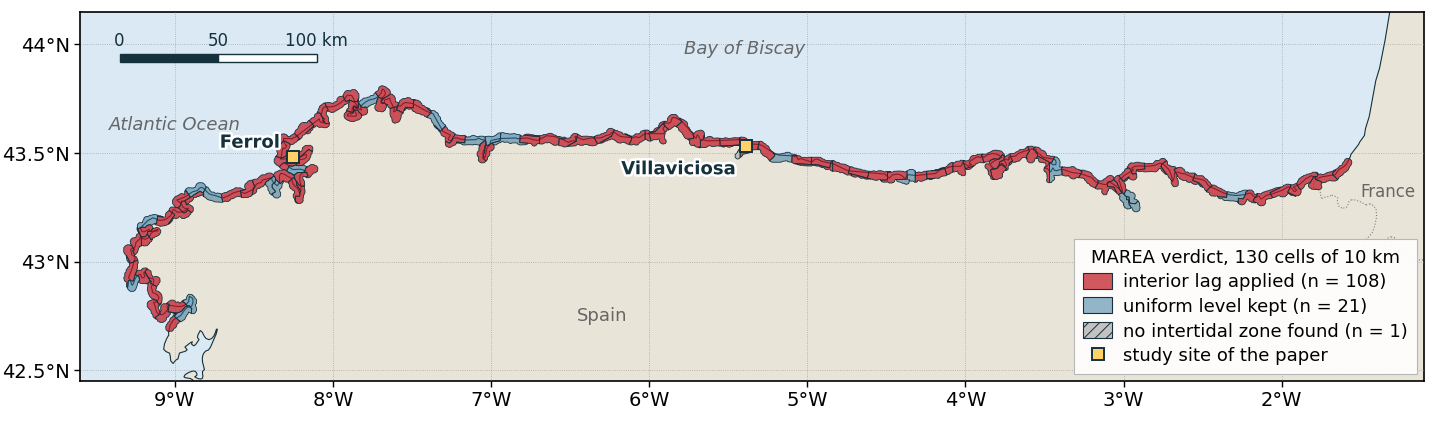
\includegraphics[width=0.9\textwidth]{fig_census.png}
\caption{The north-coast campaign: 130 cells of 10~km along the
Cantabrian and Galician coast of Spain, coloured by the verdict of the
unattended run (interior lag applied, or uniform level kept), with the
two Spanish study sites marked.}
\label{fig:census}
\end{figure*}

\subsubsection{Sentinel-2 archive}

All imagery is Sentinel-2 Level-2A surface reflectance \cite{drusch2012},
processed with Sen2Cor \cite{mainknorn2017}, from the Copernicus Data
Space Ecosystem via openEO. Every acquisition of the period, with no
cloud selection, enters a datacube of three layers per scene, the bands
B03 (green) and B08 (near-infrared) at their native 10~m and the scene
classification layer SCL; Villaviciosa and Ferrol stay at 10~m, the
much larger Dutch sites are resampled to 20~m at download. The water
index is the NDWI of McFeeters~\cite{mcfeeters1996},
$(\mathrm{B03}-\mathrm{B08})/(\mathrm{B03}+\mathrm{B08})$, preferred to
its short-wave infrared variant \cite{xu2006} because both bands are
native 10~m and SWIR indices read wet sediment as water
\cite{bishoptaylor2019waterline,bishoptaylor2026}. Acquisition instants
come from the catalogue metadata, not the nominal overpass time; the
difference reaches minutes, hence centimetres of tide.

One openEO batch job per site builds the cube once, server-side; every
later stage of the released library streams it from disk in time blocks
of bounded memory, so a ten-year archive fits a laptop and cells run in
parallel. Scenes are screened by the cloudy share of the
transition zone, the pixels neither always land nor always water, not
of the whole frame, and within a kept scene every cloudy pixel is
masked by the scene classification (Fig.~\ref{fig:clouds}): a cloud
over the hills costs nothing, a cloud over the flat costs observations,
not the scene. At Villaviciosa 305 of 1\,379 scenes pass the 10\,\%
rule over the transition zone; the same rule over the frame would keep
307, but a different set: 25 scenes with a cloudy frame and a clear
flat enter, 27 with a clear frame and a cloudy flat leave. On the Dutch
frames, mostly sea and flat, the two rules nearly coincide (66 against
67 scenes on the Westerschelde, 48 against 45 on the Ems); there the
frame rule left the comparison method 11 rising scenes on the
Westerschelde, one short of the 12 its fit needs.

\begin{figure*}[t]
\centering
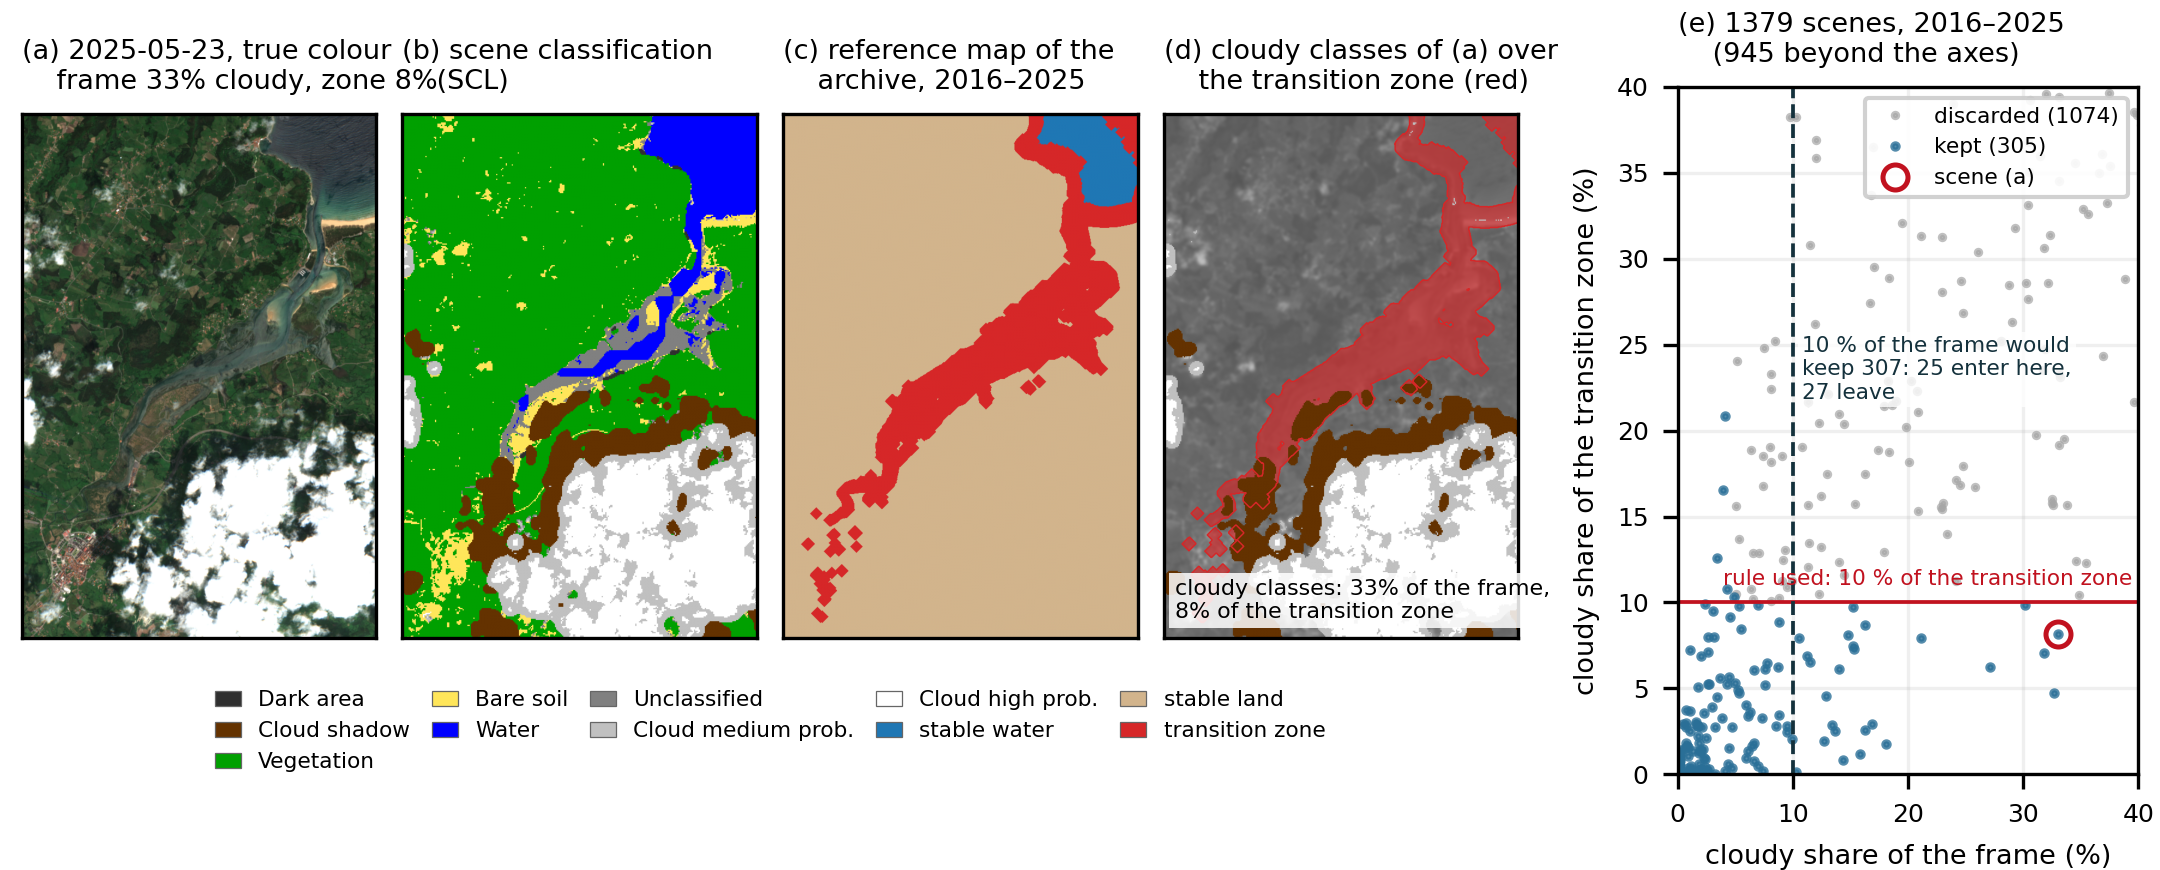
\includegraphics[width=0.92\textwidth]{fig_clouds.png}
\caption{Cloud screening over the transition zone, R\'ia de
Villaviciosa. (a) A kept scene in true colour, clouds over the hills and
a clear r\'ia; (b) its Sentinel-2 scene classification; (c) the
reference map of the archive: stable water, stable land and the
transition zone between them, the only pixels the screening looks at;
(d) the cloud mask of that scene laid over the transition zone: the
share of the zone under cloud is what the rule reads; (e) every scene of
the archive by the cloudy share of the frame and of the transition zone,
with the 10\,\% rules and the number of scenes each keeps.}
\label{fig:clouds}
\end{figure*}

\subsubsection{Tides}

The ocean boundary is EOT20 \cite{hartdavis2021}, evaluated with pyTMD
\cite{sutterley2025,fitzpatrick2024} at a fixed point in each mouth
channel at each acquisition instant. Tide-gauge records, minute-scale
for 2023--2025 from the IOC Sea Level Station Monitoring Facility
\cite{ioc2026}, are cleaned of spikes and outliers by a rolling-median
rule, demeaned, and left with their gaps over one hour open; the
Vlissingen record is missing for eighteen months. A boundary is the
model alone, the $N$ nearest gauges with inverse-square-distance
weights, or their consensus, the plain mean of two; the choice is
stated with every result, and a site's judge gauge never enters its
boundary.

\subsubsection{Elevation truth}

For the Dutch sites the truth is the Vaklodingen of Rijkswaterstaat
\cite{rws_vaklodingen}, grids from echo-sounding and airborne laser
altimetry at 20~m relative to NAP; 32 sheets of different survey years
cover the three sites, the Dollard last in 2020. For Villaviciosa it is
an RTK-GNSS survey: 361 fixed solutions of 1.3~cm nominal precision
along a 0.75~km transect at the lowest spring tide of the month. Before
any elevation product existed, 35\,\% of the surveyed pixel blocks were
sealed under a runtime guard; all numbers here use the development
subset. The 5~m national LiDAR (PNOA) is a second reference at the two
Spanish sites, with the caveat of Section~\ref{sec:validation}: over
the flats it records the water surface at flight time. All truths are
in datums other than the tide model's, so every comparison removes and
reports the median offset.

\begin{figure*}[t]
\centering
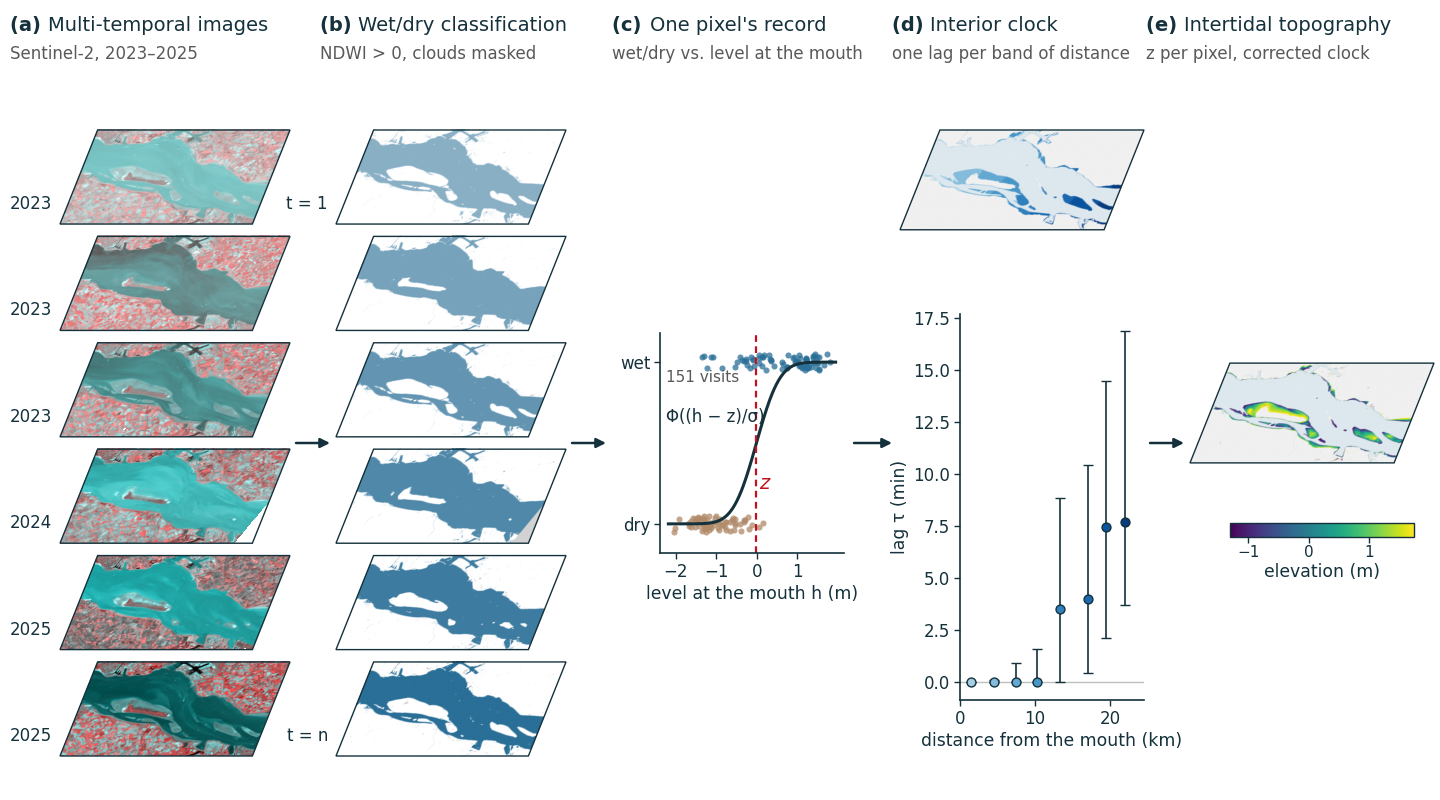
\includegraphics[width=0.88\textwidth]{fig_pipeline.png}
\caption{The pipeline on the Westerschelde, 2023--2025. (a) Dated
scenes of the archive; (b) each scene reduced to wet/dry, NDWI above
the threshold on clear-sky pixels; (c) one pixel's record against the
water level at the mouth at each visit, with its fitted transition;
(d) the interior clock: bands of geodesic distance from the mouth and
one lag per band with its bootstrap interval; (e) the elevation map,
inverted pixel by pixel on the corrected clock.}
\label{fig:pipeline}
\end{figure*}

\begin{figure*}[t]
\centering
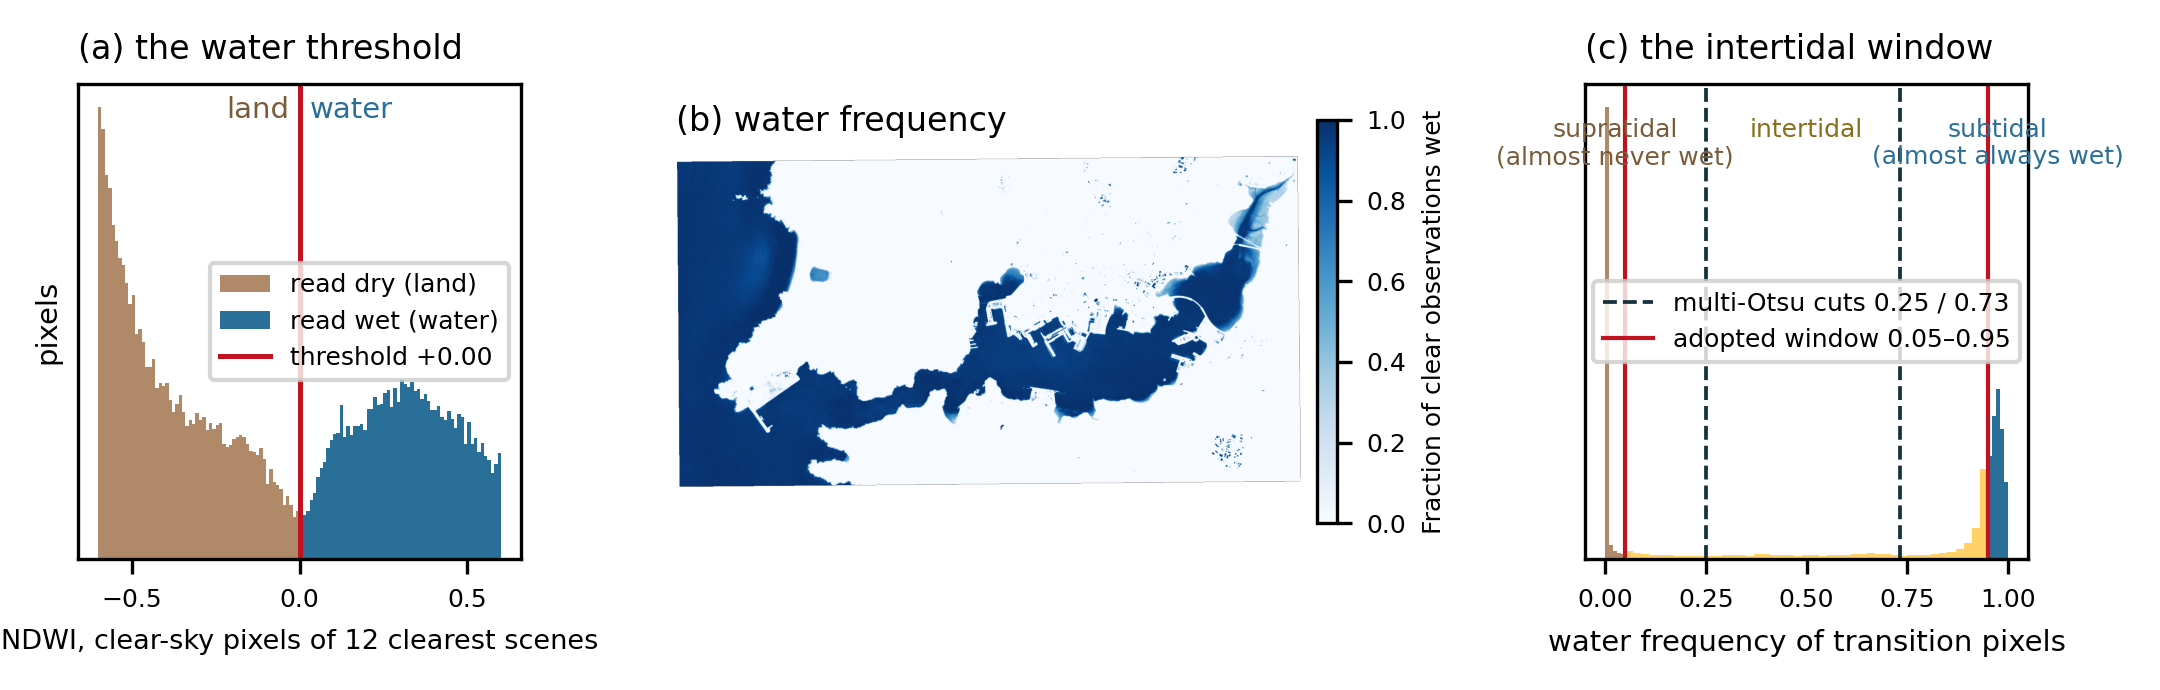
\includegraphics[width=0.86\textwidth]{fig_water.png}
\caption{Water detection on the R\'ia de Ferrol, 2023--2025. (a) NDWI
of the clear-sky pixels of the twelve clearest scenes and the adopted
threshold: land dominates the histogram and turbid estuarine water sits
below the textbook 0.1, so the split is set at 0 at every site; (b) the
water frequency, framed by the study polygon; (c) the water frequency
of the transition pixels, the multi-Otsu cuts between the three classes
and the adopted window, wider than the cuts because the surveyed flats
of Villaviciosa lie mostly in the rarely wet class
(Section~\ref{sec:pixel}).}
\label{fig:water}
\end{figure*}

% Draft of Sections 2.2-2.5 (Methods). Body text only; to be pasted into
% main.tex in place of the four "(to be written)" placeholders.
% Sources: docs/METHOD.md, docs/one_pixel_marea_example.md,
% docs/tide_adjustment_comparison.md (1, 5), docs/prior_art_granadeiro.md,
% pyintertidal/marea.py, pyintertidal/tide_estimators.py,
% pyintertidal/elevation.py, configs/m2.yaml, experiments/sota_granadeiro.py,
% experiments/e0_escalda_prep.py.

\subsection{The pixel model and the elevation inversion}\label{sec:pixel}

For a shoreline pixel with flooded fraction $f$, linear mixing of the
McFeeters water index~\cite{mcfeeters1996} gives
\begin{equation}\label{eq:mix}
\mathrm{NDWI} = (1-f)\,\mathrm{NDWI}_{\mathrm{dry}} + f\,\mathrm{NDWI}_{\mathrm{wet}}
= a + b\,f ,
\end{equation}
where the dry level $a$ and the dry-to-wet jump $b$ are fitted per
pixel, which normalises albedo between pixels. At water level $h$,
$f(h) = \Pr(\text{internal elevation} \le h)$ is the cumulative
distribution of the pixel's relief, assumed Gaussian with mean $z$, its
median elevation, and spread $\sigma$, its roughness:
\begin{equation}\label{eq:pixel}
\mathrm{NDWI}(h) = a + b\,\Phi\!\left(\frac{h - z}{\sigma}\right),
\end{equation}
with $\Phi(u) = (2\pi)^{-1/2}\int_{-\infty}^{u} e^{-v^{2}/2}\,\mathrm{d}v$
the standard normal distribution function; the midpoint $h = z$ is the
elevation. Eq.~\eqref{eq:pixel} is the probit ogive of
quantal-response analysis \cite{bliss1934,finney1947}, the Gaussian
counterpart of the per-pixel methods' logistic \cite{berkson1944}. The
fitted $\sigma$ also absorbs the water-level error of each scene.

The inversion (\texttt{invert\_series}) fits Eq.~\eqref{eq:pixel} to
each pixel's clear observations by least squares: for each candidate
$(z, \sigma)$ the linear $(a, b)$ is solved in closed form, $z$ runs
over 50 points between the lowest and highest level of the series,
$\sigma$ over the archive's eight relief atoms (0.03, 0.06, 0.10, 0.15,
0.22, 0.32, 0.45 and 0.65~m), and the pair with the smallest residual is
kept. A pixel is left blank with fewer than 8 clear observations, a
contrast $b$ outside $(0.15, 2.5)$ or a dry level $|a| \ge 2.5$.

A scene is kept if at most 10\,\% of the transition zone is cloudy; an
observation is used only where Sen2Cor reads vegetation, bare ground or
water (the campaign extraction also admits unclassified). The wet/dry
label is $\mathrm{NDWI} > 0$: Otsu's threshold \cite{otsu1979} on the
twelve clearest development-site scenes lands at $+0.25$, the top of its
allowed range; zero is preferred because turbid estuarine water reads
lower than clear water. The intertidal zone is delimited by water
frequency, the wet fraction of a pixel's clear observations. A
three-class Otsu split of the transition pixels separates ground, flat
and channel, with valleys at 0.21 and 0.66 in Villaviciosa, and
confirms that the archive holds three populations; but the flats reach
far into the rarely wet class: of the 181 intertidal pixels the
development RTK survey covers, only 79 lie inside the Otsu window
against 130 inside 0.05--0.95. The window is therefore set by what the
inversion
can resolve, a pixel with enough clear observations on both sides of
its transition, and opened to 0.05--0.95. The four test-site products
use the fixed window and minimum count of Section~\ref{sec:sites}. Elevations are fitted within an epoch,
2023--2025 for the products of Section~\ref{sec:results}.

\subsection{The interior clock}\label{sec:clock}

The interior tide is measured per band of along-channel distance $s$
from the mouth: $s$ is the geodesic distance, the minimum-cost
eight-connected path over the permanent-water and intertidal masks
times the pixel size, from the permanent-water pixels (water frequency
at least 0.90) on the image border on the sides declared as sea.
Intertidal pixels are split into 3-km bands along $s$; a band with fewer
than 500 pixels is merged with the next. Each band sits at the median
$s$ of its pixels, and at most 1\,200 of them, drawn at random with a
fixed seed, enter the likelihood.

% fig:method removed from the paper (its panels are in the pipeline and
% likelihood figures); experiments/paper_fig_method.py is kept.


Each observation is reduced to its binary label $y_{pt} \in \{0,1\}$ and
the amplitudes of Eq.~\eqref{eq:pixel} are fixed at 0 and 1, leaving two
parameters per pixel: a Rasch-type model \cite{rasch1960,engelhard2021}
(scenes as persons, pixels as items). Under a candidate clock $\tau_k$
for band $k$ the level at scene $t$ is $h(t-\tau_k)$, pixel $p$ is wet
with probability $P_{pt} = \Phi\big((h(t-\tau_k) - z_p)/\sigma_p\big)$,
and the profiled Bernoulli log-likelihood of the band is
\begin{equation}\label{eq:profile}
\ell_k(\tau_k) = \sum_{p \in k}\; \max_{z_p,\,\sigma_p}\; \sum_{t}
\Big[\, y_{pt}\log P_{pt} + (1-y_{pt})\log(1-P_{pt}) \Big],
\end{equation}
where $t$ runs over the pixel's clear scenes. The inner maximum is the
profiling of variable projection \cite{golub1973,kaufman1975}: every
pixel re-fits its own $(z_p, \sigma_p)$ under each clock, so clocks are
decided only by what terrain cannot absorb, the reordering of the tide
across dates (Fig.~\ref{fig:likelihood}). The grid is 60 points of $z_p$
over the boundary's tidal range plus 0.3~m on either side, about 8~cm
apart, and, in the product, the six interior relief atoms, 0.06 to
0.45~m, for $\sigma_p$; probabilities are clipped at $10^{-4}$, and a
pixel needs at least six clear scenes.

The boundary is evaluated once at every acquisition instant shifted by
the sixteen values $-45, -30, \ldots, 180$~min of the shift bank, and
$h(t-\tau)$ is interpolated linearly between them. The mouth band is
pinned at $\tau_0 = 0$. The free parameters are the increments between
successive bands, $\tau_k = \sum_{j \le k} \delta_j$ with every
$\delta_j \ge 0$, so the profile is monotone non-decreasing inland. The
negative of Eq.~\eqref{eq:profile}, summed over bands and normalised per
observation, is minimised with L-BFGS-B \cite{byrd1995} in SciPy
\cite{virtanen2020}, the increments in hours, bounded between 0 and
$+180$~min and started at zero.

\begin{figure*}[t]
\centering
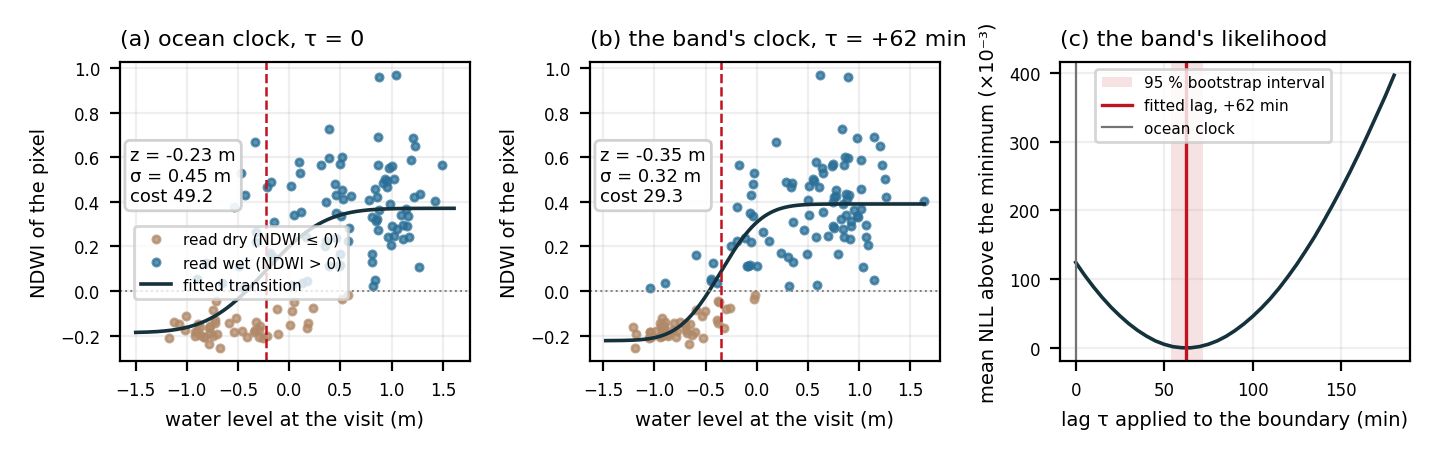
\includegraphics[width=0.86\textwidth]{fig_likelihood.png}
\caption{What the clock does to the likelihood, on the Ems-Dollard band
containing the Delfzijl gauge. (a) One pixel of the band on the ocean
clock: its NDWI at each visit against the water level at the mouth,
coloured by the reading (wet above 0, dry below), and the transition
$a + b\,\Phi((h - z)/\sigma)$ with the $(z, \sigma)$ profiled by the
binary likelihood; wet and dry readings overlap over a wide range of
levels. (b) The same pixel on the band's clock: the readings separate,
the transition sharpens and the pixel's negative log-likelihood (cost)
falls. (c) The band's profiled
negative log-likelihood against the lag, relative to its minimum, with
the fitted lag, its 95\,\% bootstrap interval and the ocean clock.}
\label{fig:likelihood}
\end{figure*}

\subsection{Identifiability and adoption}\label{sec:adoption}

The interior tide may also be amplified or damped: with a gain $\alpha$
and a datum shift, $h_{\mathrm{int}}(t) = \alpha\,h(t-\tau) + \mathrm{datum}$.
Binary data cannot read $\alpha$: with $P = \Phi\big((\alpha h - z)/\sigma\big)$,
multiplying $\alpha$, $z$ and $\sigma$ by one constant $c$ gives
\begin{equation}\label{eq:affine}
\frac{(c\alpha)\,h - (cz)}{c\sigma} = \frac{\alpha h - z}{\sigma},
\end{equation}
so the likelihood is unchanged, and a datum shift is absorbed by $z$.
Only the phase survives, so it is measured from the imagery; gain and
datum come from the boundary. The check is executable: with a gain of
1.0--1.3 planted in the simulator, the negative log-likelihood profile
in $\alpha$, with $(z, \sigma)$ profiled on grids scaling with $\alpha$,
must be flat.

Each band lag carries a scene-bootstrap interval: the scenes are
resampled with replacement thirty times, the profile refitted on each,
and the 2.5th and 97.5th percentiles of the thirty $\tau_k$ are its
95\,\% confidence interval; an interval containing zero means the lag is
not distinguishable from none. No threshold is applied and no lag
discarded; the interval says which values carry information. On replica
archives with the pixels, cloud masks and acquisition instants of a real
site but a uniform tide with no interior lag, the estimator returns lags
of the order of ten minutes; the experiments are released with the code.

Each pixel receives the band profile smoothed along $s$ with a Gaussian
kernel of the band length, anchored at $\tau = 0$ at the mouth and kept
monotone, evaluated at the pixel's own distance and rounded to the
minute. The inversion of Section~\ref{sec:pixel} is then run once with
the boundary evaluated at the exactly shifted instants $t - \tau$, not
the bank's 15-min interpolation, and the $z$ grid spanning the unshifted
boundary range everywhere. The product stores the band lags, their
intervals and the lag every pixel received.

\subsection{The comparison method}\label{sec:granadeiro}

The elevation maps are compared with those of the published method of
Granadeiro et al.~\cite{granadeiro2021}, which fits a logistic with
four parameters to standardised near-infrared reflectance against water
height
per pixel, the inflection being the elevation, and reads a tidal-stage
lag per pixel from the disagreement between its rising and ebbing fits,
extended over the flat by a thin-plate spline. It was reimplemented from
the paper, not their code, with SciPy \cite{virtanen2020} for the fits,
and run on the same pixels, scenes and boundary as MAREA; the
reimplementation and its declared substitutions are released with the
code.


% Validation (2.6) and the whole of Section 3 (results skeleton); the
% numbers in its tables are refilled from the notebook outputs after each
% re-execution of the pipeline.
% Validation subsection (2.6) and Section 3, \input by main.tex.
% Every number must trace to the CSVs the pipeline notebooks write
% (tide_boundary_comparison_<site>.ipynb sections 10/10b,
% intertidal_topography_villaviciosa.ipynb sections 9a/9b); the scripts
% experiments/v4_lag_external.py, v5_rtk_onsite.py and v6_lidar_external.py
% only assemble them into results/*.json and the paper figures.
% Convention: "MAREA's lag at the inner gauge" is the smoothed band profile
% evaluated at the gauge's distance from the mouth, i.e. what a pixel there
% receives; the band that contains the gauge and its 95 % interval are
% given beside it. The comparison method's lag is not scored against gauges.
% Runs of 2026-09-23 (fixed-band product): Ferrol, Westerschelde, Ems and
% Wadden done; Villaviciosa (RTK, LiDAR) pending -> \ldots.

\subsection{Validation}\label{sec:validation}

The method yields two quantities, the lag of each band and the elevation
of each pixel, each validated on site, in the R\'ia de Villaviciosa, and
externally, against tide-gauge records and surveys made by others
(Table~\ref{tab:validation}). The lag blocks ask whether the measured
lag is real and whether applying it improves the level assigned inside
the estuary; the elevation blocks set both maps against independent
surveys. Nothing that judges a result enters a fit.

\begin{table*}[t]
\centering
\caption{The four validation blocks: what is validated, against what,
where, and with which metric.}
\label{tab:validation}
\footnotesize
\setlength{\tabcolsep}{5pt}
\resizebox{\textwidth}{!}{%
\begin{tabular}{@{}llll@{}}
\toprule
block & reference & sites & metric \\
\midrule
lag, on site & pressure sensors along the r\'ia & Villaviciosa & lag in reaching the same level (min); \\
 & (campaign pending) & & same-instant level difference (m) \\
lag, external & gauge pair: mouth and inner (judge) & Ferrol, Westerschelde, & gauge-pair lag vs.\ lag applied (min); \\
 & & Ems-Dollard, Wadden & RMSE of the level at the judge, without \\
 & & & and with the lag (m) \\
elevation, on site & RTK-GNSS survey, development split & Villaviciosa & RMSE, slope $b$, $r$ of each map on the \\
 & & & survey (Eq.~\ref{eq:metrics}); transect profile \\
elevation, external & IGN LiDAR DTM; Vaklodingen & Spanish sites; Dutch sites & RMSE, slope $b$, $r$ (Eq.~\ref{eq:metrics}), \\
 & & & by band for the Vaklodingen \\
\bottomrule
\end{tabular}}
\end{table*}

\subsubsection{Metrics and the datum}

Lags are compared in minutes: the gauge-pair lag is the mean over
paired tidal cycles $c$ of $t^{\mathrm{in}}_c - t^{\mathrm{mouth}}_c$,
the instants at which the inner and the mouth record cross the same
level on the same limb, and it is set against the lag MAREA applies at
the inner gauge. The effect of a lag on the water level is the RMSE
between the level a product predicts there, the boundary $h_B$ read
$\tau$ minutes earlier, and the level $h^{\mathrm{in}}$ the gauge
recorded, the median of the difference (the datum) removed:
\begin{align}
\mathrm{RMSE}_h &= \sqrt{\frac{1}{N}\sum_{t}\big(d(t) - \operatorname{median}\,d\big)^{2}}, \nonumber \\
d(t) &= h_B(t - \tau) - h^{\mathrm{in}}(t),
\label{eq:judge}
\end{align}
over the $N$ ten-minute samples of 2023--2025. Elevations are compared
with Eq.~\eqref{eq:metrics}. Products are on the datum of the tide model at
the mouth, the mean sea level of EOT20 \cite{hartdavis2021}; each truth
is on its own: NAP for the Vaklodingen \cite{rws_vaklodingen}, the
ellipsoid for the RTK-GNSS survey, orthometric heights for the LiDAR. No
method can see the constant between the two, so every comparison removes
it and reports it as the bias. On the $n$ samples where product $z$ and
truth $z^{\mathrm{t}}$ are both finite, each series is centred on its own
median, $y_i = z_i - \operatorname{median}(z)$ and
$x_i = z^{\mathrm{t}}_i - \operatorname{median}(z^{\mathrm{t}})$, and
\begin{align}
\mathrm{RMSE} &= \sqrt{\frac{1}{n}\sum_{i=1}^{n}(y_i - x_i)^2}, \qquad
b = \frac{\sum_i (x_i-\bar x)(y_i-\bar y)}{\sum_i (x_i-\bar x)^2}, \nonumber \\
r &= \frac{\sum_i (x_i-\bar x)(y_i-\bar y)}
         {\sqrt{\sum_i (x_i-\bar x)^2\,\sum_i (y_i-\bar y)^2}},
\label{eq:metrics}
\end{align}
with the truth on the abscissa: the slope $b$ says whether the map
reproduces the relief (1) or compresses it (below 1), $r$ how much of it
the map explains. Only truth within the range of scene levels, widened
by $\pm 0.25$~m, is scored: no waterline method can represent a channel
bed at $-8$~m beside a flat. A $5 \times 5$ thinning of the grid, one
pixel per 100~m block, changed no ranking.

\subsubsection{The interior lag on site: pressure sensors along the r\'ia}

The R\'ia de Villaviciosa has no interior tide gauge, so its lag will be
measured directly: absolute pressure sensors at three to four stations,
submerged through the lowest spring low water, with a barometer on land,
over 29 days at 1 to 5~min. Level follows
$h = z_s + (p - p_{\mathrm{atm}})/(\rho g)$, with $\rho = 1025$~kg\,m$^{-3}$
and $z_s$ the sensor elevation from RTK-GNSS. Each station is then
scored against the mouth as the gauge pairs below. The campaign is
pending.

\subsubsection{The interior lag against gauge pairs}

Four estuaries have a gauge near the mouth and another inside, the judge
of Section~\ref{sec:sites}: Ferrol1 and Ferrol2, Vlissingen and
Terneuzen, Borkum and Delfzijl, Terschelling Noordzee and Harlingen. Two quantities need
only the two records \cite{ioc2026}, 2023--2025, 10-min grid, demeaned,
gaps over one hour left open. The first is the lag in reaching the same
level: crossings of the 25th, 50th and 75th percentile of the mouth's
level are interpolated between samples and paired with the nearest inner
crossing within three hours; their mean difference over paired cycles,
and per limb, is the gauge-pair lag. It is compared with the lag MAREA
applies at the gauge's distance and with the 95\,\% bootstrap interval of
the band containing the inner gauge, measured from band 0, which holds
the mouth gauge (\emph{no delay}: 0 everywhere). The second is the
same-instant level difference, inner minus mouth: its RMS and mean are
the error of the uniform level every published method assumes. The third
is the level predicted at the inner gauge from the mouth boundary read
$\tau$ minutes earlier, with $\tau = 0$ and with MAREA's lag there,
scored on the gauge's record as the median-centred RMSE of
Eq.~\eqref{eq:metrics}. Nothing was fitted on the inner gauge, so the
whole record is the test. The comparison method's lag, per pixel over
the flats, reaches no gauge and is scored only through its elevations.

\subsubsection{Elevation on site: the RTK-GNSS survey}

In Villaviciosa the maps are scored on the development subset of the
RTK-GNSS survey of Section~\ref{sec:sites}: 35\,\% of its 150~m blocks,
drawn once with a fixed seed and sealed before any elevation product
existed, released by a runtime guard only to the verdict script. The two
maps share record, epoch (2023--2025) and boundary (EOT20 at the mouth):
\emph{MAREA}, our inversion with the smoothed band profile at each
pixel's distance, and \emph{Granadeiro}, the method of
Section~\ref{sec:granadeiro} with its own lag map. Both are scored with
Eq.~\eqref{eq:metrics} and drawn with the survey along a straight
stretch of the walked route.

\subsubsection{Elevation external: the national LiDAR and the Vaklodingen}

At the Spanish sites, Villaviciosa and Ferrol, the reference is the 5~m
LiDAR DTM of the Instituto Geogr\'afico Nacional (PNOA),
% TODO: add a bib entry for the IGN MDT05 / PNOA-LiDAR product
resampled bilinearly onto the product grid; at the Dutch sites, the
Rijkswaterstaat Vaklodingen \cite{rws_vaklodingen}, yearly bathymetry
and intertidal topography on a 20~m grid (NAP), each pixel taking its
nearest cell's latest survey of 2019--2025. Both maps are scored with
Eq.~\eqref{eq:metrics} on the intertidal pixels each resolves and on
those both resolve, the Vaklodingen also by band of distance from the
mouth. A LiDAR flown at high water records the water surface over the
flats, so each LiDAR score comes with the water share of its truth: the
share of intertidal cells within 5~cm of the modal value.

\section{Results and discussion}\label{sec:results}

\subsection{The interior lag against the gauge pairs}\label{sec:res_lag}

\begin{table*}[t]
\centering
\caption{The interior lag against the gauge pairs, 2023--2025. Lag between
the mouth gauge and the inner gauge in reaching the same level (mean over
paired cycles and limbs, positive: the inner gauge is later); lag MAREA
applies at the inner gauge, with the 95\,\% bootstrap interval of its
band; RMS difference between the two gauge records at the same instant,
the error of copying the mouth gauge inland; and the RMSE of the level
predicted at the inner gauge from the boundary the products use (the
consensus of EOT20 and the mouth gauge), without and with the lag.
% NUMBERS: lag_pair_metrics.csv and judge_metrics.csv of each site's
% comparison notebook, run of 2026-09-23.
}
\label{tab:lag_external}
\footnotesize
\setlength{\tabcolsep}{6pt}
\begin{tabular}{@{}lrrrr@{}}
\toprule
 & lag between & lag applied & inner vs.\ mouth gauge, & level at the inner gauge from \\
site (inner gauge, km from mouth) & gauges (min) & by MAREA (min) & same instant, RMS (m) & the boundary (m): no lag $\to$ MAREA \\
\midrule
Ferrol (Ferrol2, 10.1) & $+4$ & $0$ $[0, +2]$ & 0.10 & $0.112 \to 0.112$ \\
Westerschelde (Terneuzen, 21.9) & $+19$ & $+7$ $[+4, +17]$ & 0.28 & $0.356 \to 0.311$ \\
Ems-Dollard (Delfzijl, 24.4) & $+51$ & $+63$ $[+54, +72]$ & 0.50 & $0.620 \to 0.358$ \\
Wadden, Vlie (Harlingen, 18.3) & $+88$ & $+129$ $[+123, +138]$ & 0.53 & $0.562 \to 0.303$ \\
\bottomrule
\end{tabular}
\end{table*}

% figure fig:lag_external is placed after the bibliography (main.tex)


% Numbers: lag_pair_metrics.csv and judge_metrics.csv of each site (run of
% 2026-09-23).
The gauge pairs order the sites as the archive does
(Table~\ref{tab:lag_external}, Fig.~\ref{fig:lag_external}). In Ferrol
the inner gauge lags the mouth by 4~min and one level for the whole
r\'ia errs by 0.10~m RMS; MAREA measures 0~min there, interval 0 to
$+2$, and the level error stays at 0.112~m. In the Westerschelde the
gauges are 19~min apart on both limbs; MAREA applies $+7$~min at
Terneuzen, the band's interval reaching $+17$, and the error falls from
0.356 to 0.311~m. In the Ems-Dollard the lag is 51~min, 41 rising and 61
falling; MAREA applies $+63$~min at Delfzijl, inside its interval of
$+54$ to $+72$, and the error falls from 0.620 to 0.358~m, by 42\,\%. In
the Vlie basin the gauges are 88~min apart, 91 rising and 85 falling;
MAREA applies $+129$~min at Harlingen, interval $+123$ to $+138$, 41~min
beyond the gauges, and the error still falls from 0.562 to 0.303~m, by
46\,\%. Two columns of Table~\ref{tab:lag_external} differ in kind: the
same-instant difference sets the two gauge records against each other,
whereas the level error is that of the boundary the products read, the
consensus of EOT20 and the mouth gauge, which adds the model's error to
the uniform-level assumption; hence the boundary without a lag (0.620~m
in the Ems-Dollard) is worse than the mouth gauge copied inland
(0.50~m), and MAREA with the lag (0.358~m) beats either. Where an
interior tide exists the archive measures it; where none exists it
applies the few minutes its intervals declare, at a cost of centimetres
at most.

\subsection{Elevation against the RTK survey}\label{sec:res_rtk}

\begin{table}[t]
\centering
\caption{Elevation against the RTK-GNSS survey, Villaviciosa development
subset, 2023--2025, EOT20 boundary. $n$: surveyed points the map
resolves; RMSE, slope $b$ and $r$ as in Eq.~\eqref{eq:metrics}, RTK on
the abscissa; bias: the datum offset, ellipsoidal heights against the
tide-model datum, removed before scoring.
% NUMBERS: products_marea/rtk_onsite_metrics.csv (Villaviciosa notebook,
% section 9a), run pending.
}
\label{tab:rtk}
\footnotesize
\begin{tabular}{@{}lrrrrr@{}}
\toprule
method & $n$ & RMSE (m) & $b$ & $r$ & bias (m) \\
\midrule
MAREA & 194 & 0.193 & 0.72 & 0.86 & $-52.8$ \\
Granadeiro & 163 & 0.275 & 0.39 & 0.63 & $-53.3$ \\
\bottomrule
\end{tabular}
\end{table}

% figure fig:rtk_onsite is placed after the bibliography (main.tex)



% Numbers: products_marea/rtk_onsite_metrics.csv (section 9a of the
% Villaviciosa notebook; experiments/v5_rtk_onsite.py runs the same code).
On the 194 surveyed points it resolves, MAREA reaches 0.193~m RMSE with
slope 0.72 and $r = 0.86$; the Granadeiro map reaches 0.275~m with
slope 0.39 and $r = 0.63$ on 163 points (Table~\ref{tab:rtk},
Fig.~\ref{fig:rtk_onsite}a,b). Along a straight 192-m stretch of the
walked route
(Fig.~\ref{fig:rtk_onsite}c--e) the MAREA profile follows the survey
within the pixel size, including the fall at its inland end, where the
Granadeiro profile stays flat. The lag applied on the surveyed pixels is
5~min in median and 16 at most, so Villaviciosa tests the estimator
more than the clock.

\subsection{Elevation against the external references}\label{sec:res_lidar}

\begin{figure*}[t]
\centering
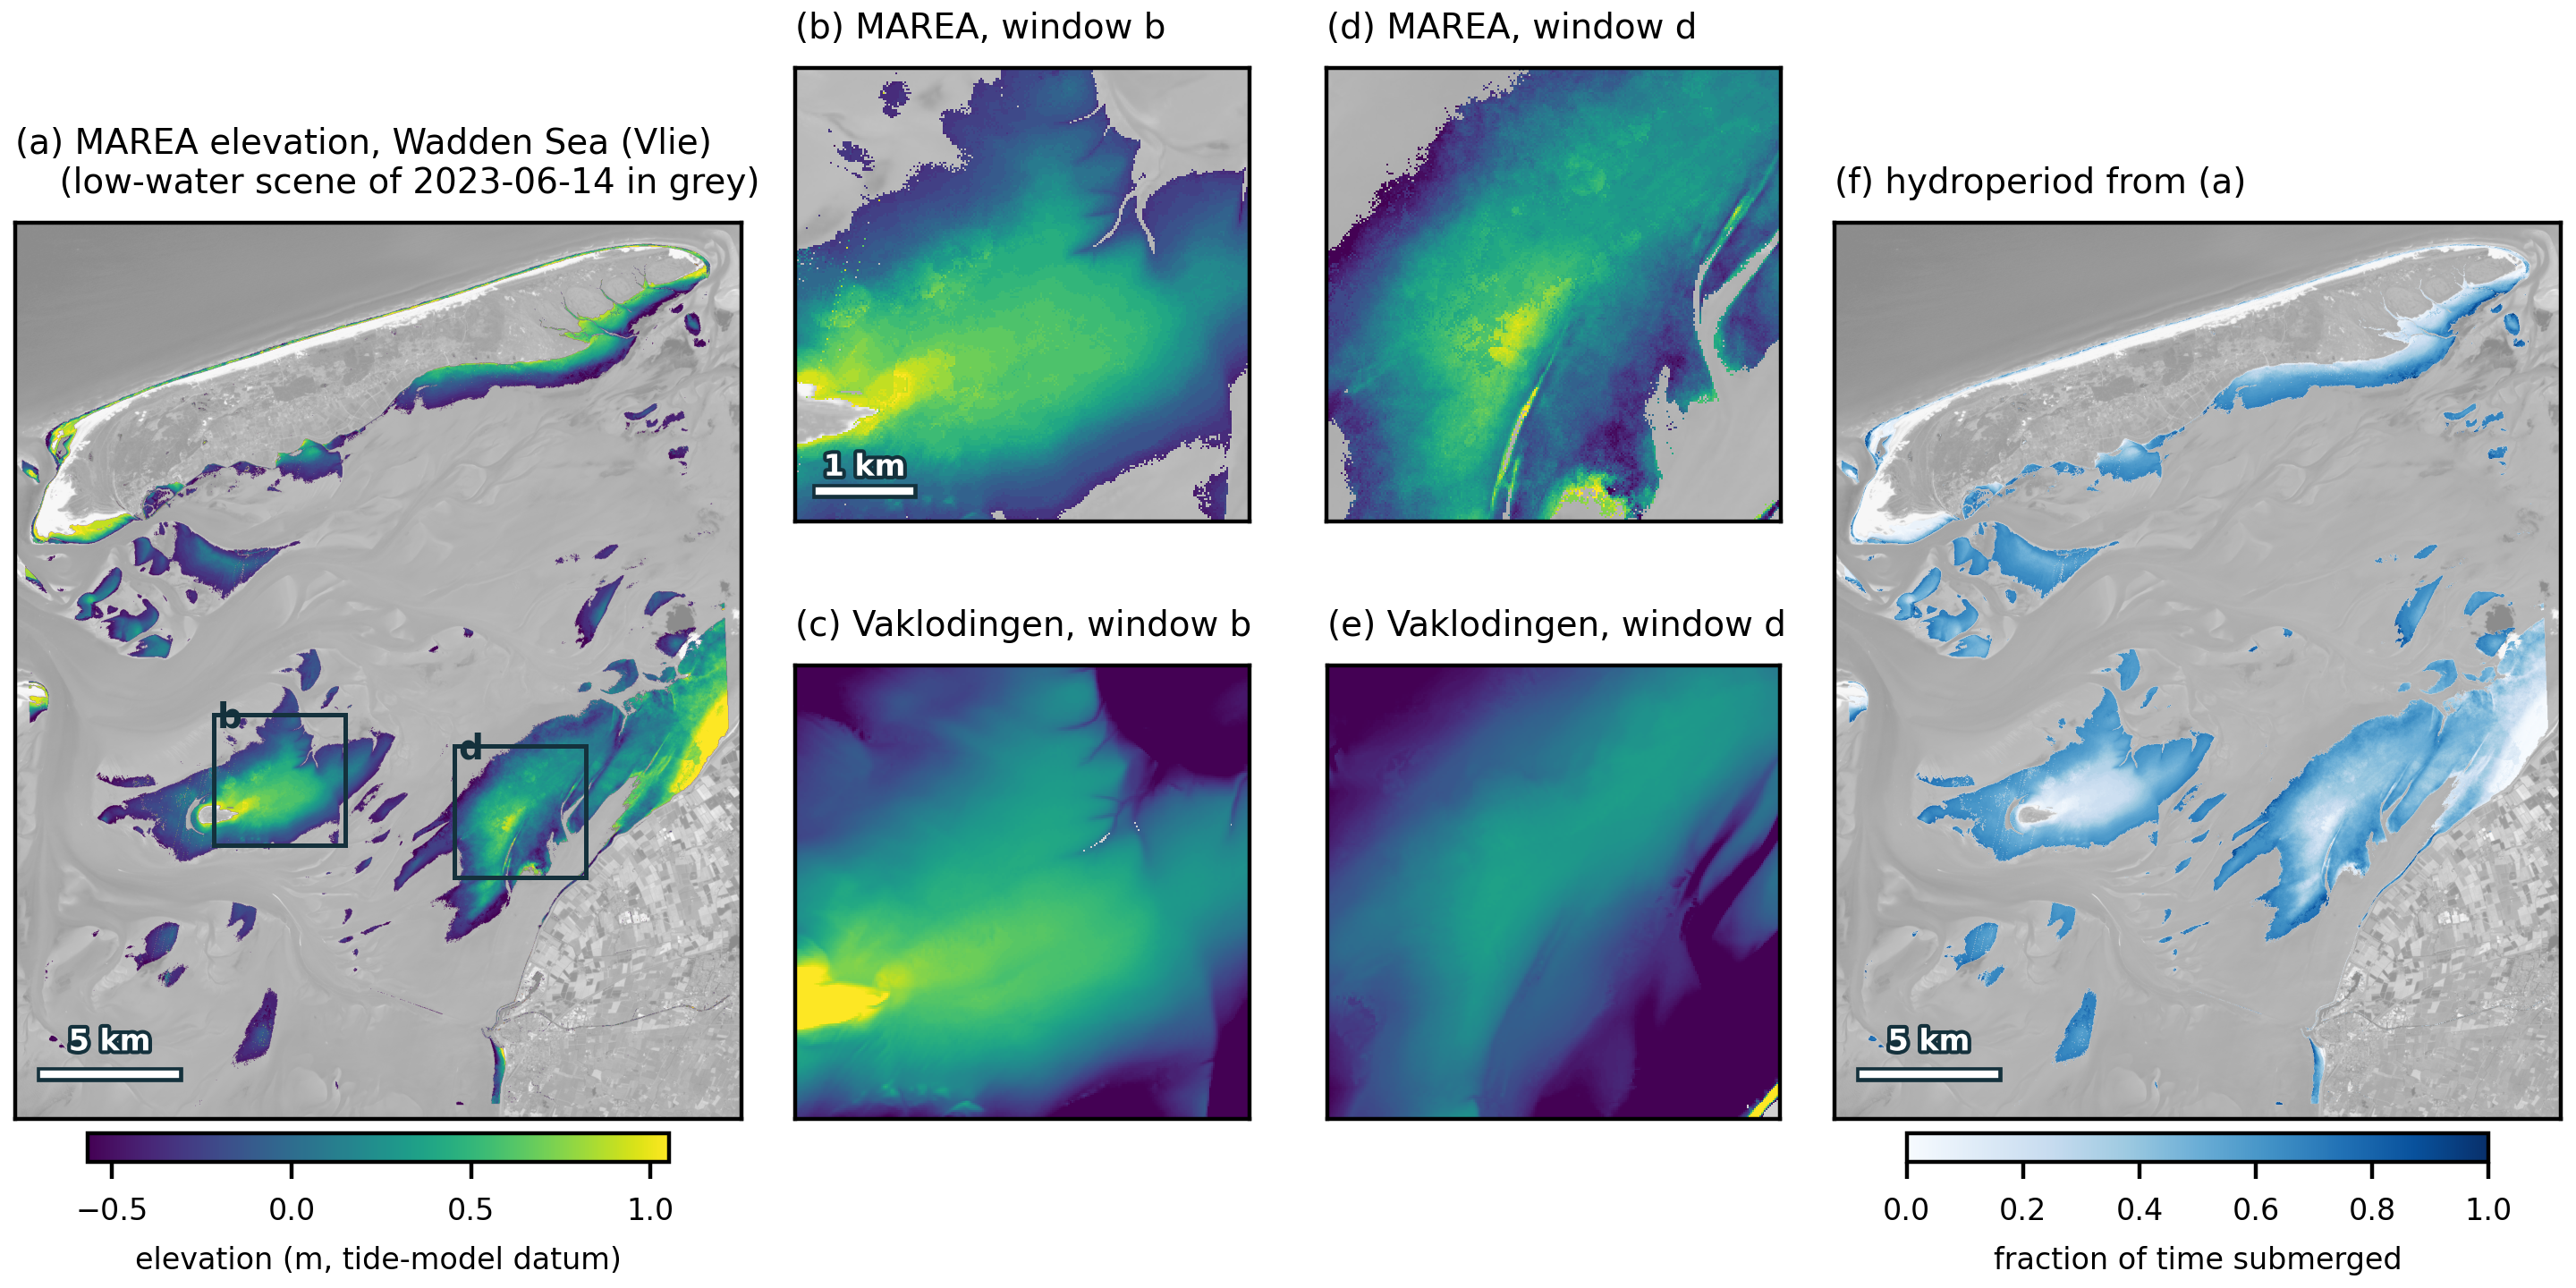
\includegraphics[width=0.94\textwidth]{fig_products.png}
\caption{The products of the Wadden Sea site (Vlie inlet to Harlingen),
2023--2025, over the clearest low-water scene of the archive in grey.
(a) The MAREA elevation map on the intertidal zone, with two zoom
windows marked; (b), (d) the windows in the MAREA map (20-m grid);
(c), (e) the same windows in the Rijkswaterstaat Vaklodingen, the
official survey of the flats and channels, one value per 20-m cell taken
cell for cell without interpolation, same colour scale, datum offset
removed; (f) the hydroperiod, the fraction of time each pixel is
submerged, from map (a) and the tide series.}
\label{fig:products}
\end{figure*}

% NUMBERS: lidar_metrics.csv (Ferrol), products_marea/lidar_external_metrics.csv
% (Villaviciosa), vaklodingen_metrics.csv / vaklodingen_by_band.csv (Dutch
% sites), run of 2026-09-23; experiments/v6_lidar_external.py assembles them.
\begin{table*}[t]
\centering
\caption{Elevation against the external references: the IGN 5~m LiDAR
DTM (PNOA) at the Spanish sites, the Rijkswaterstaat Vaklodingen at the
Dutch sites. Each map on all intertidal pixels it resolves (left) and on
those both resolve (right), Eq.~\eqref{eq:metrics}, reference inside the
tide range the maps could sample. Spanish site headers give the LiDAR
diagnostic: modal value over the intertidal mask and share of cells
within 5~cm of it, the water-surface share of the truth.}
\label{tab:external}
\footnotesize
\setlength{\tabcolsep}{4pt}
\resizebox{\textwidth}{!}{%
\begin{tabular}{@{}lrrrrrrr@{}}
\toprule
 & \multicolumn{4}{c}{all resolved pixels} & \multicolumn{3}{c}{common pixels} \\
\cmidrule(lr){2-5}\cmidrule(lr){6-8}
method & $n$ & RMSE (m) & $b$ & $r$ & RMSE (m) & $b$ & $r$ \\
\midrule
\multicolumn{8}{@{}l}{\emph{R\'ia de Villaviciosa}, IGN LiDAR --- mode $+2.00$~m, 69\,\% of cells within 5~cm, above the tide range and excluded} \\
MAREA & 7\,458 & 0.803 & 0.47 & 0.33 & 0.760 & 0.42 & -- \\
Granadeiro & 4\,477 & 0.775 & 0.32 & 0.25 & 0.767 & 0.33 & -- \\
\midrule
\multicolumn{8}{@{}l}{\emph{R\'ia de Ferrol}, IGN LiDAR --- mode $0.00$~m, 78\,\% of cells within 5~cm} \\
MAREA & 51\,716 & 0.736 & 0.46 & 0.13 & 0.648 & 0.53 & -- \\
Granadeiro & 49\,262 & 0.732 & 0.36 & 0.09 & 0.644 & 0.54 & -- \\
\midrule
\multicolumn{8}{@{}l}{\emph{Westerschelde}, Vaklodingen} \\
MAREA & 62\,181 & 0.435 & 0.76 & 0.92 & 0.385 & 0.80 & 0.94 \\
Granadeiro & 45\,005 & 0.777 & 0.78 & 0.77 & 0.776 & 0.78 & 0.78 \\
\midrule
\multicolumn{8}{@{}l}{\emph{Ems-Dollard}, Vaklodingen} \\
MAREA & 412\,565 & 0.363 & 0.65 & 0.84 & 0.327 & 0.67 & 0.86 \\
Granadeiro & 98\,953 & 0.531 & 0.39 & 0.58 & 0.521 & 0.40 & 0.58 \\
\midrule
\multicolumn{8}{@{}l}{\emph{Wadden Sea (Vlie)}, Vaklodingen} \\
MAREA & 348\,894 & 0.329 & 0.81 & 0.68 & 0.230 & 1.00 & 0.83 \\
Granadeiro & 65\,576 & 0.477 & 0.65 & 0.44 & 0.427 & 0.77 & 0.53 \\
\bottomrule
\end{tabular}}
\end{table*}

% figure fig:vaklodingen_bands is placed after the bibliography (main.tex)


% Numbers: vaklodingen_metrics.csv / vaklodingen_by_band.csv (Dutch sites),
% lidar_metrics.csv (Ferrol), run of 2026-09-23. Villaviciosa pending.
Against the Vaklodingen (Table~\ref{tab:external},
Fig.~\ref{fig:vaklodingen_bands}) MAREA is the closer map at the three
Dutch sites. In the Westerschelde it scores 0.435~m RMSE with slope 0.76
and $r = 0.92$ on 62\,000 pixels, Granadeiro 0.777~m on 45\,000. In the
Ems-Dollard MAREA scores 0.363~m with slope 0.65 and $r = 0.84$ on
413\,000 pixels; Granadeiro resolves a quarter of them at 0.531~m with
slope 0.39. In the Vlie basin MAREA scores 0.329~m with slope 0.81 on
349\,000 pixels, Granadeiro 0.477~m on 66\,000; on the pixels both
resolve, 0.230 against 0.427~m. Fig.~\ref{fig:products} shows the Vlie
map beside the Vaklodingen and the hydroperiod derived from it. The lag
carries the two large sites:
inverted without it, the same pixels score 0.565~m with slope 0.24 in
the Ems-Dollard and 0.474~m in the Vlie, and beyond 28~km of the Ems the
error falls from 0.50--0.66~m to 0.28--0.42~m with the clock.
% ^ ablation of MAREA's own clock (from the same CSVs), kept as one
% sentence; not a method row in the tables.
At the Spanish sites the LiDAR is a water surface: 78\,\% of the Ferrol
cells lie within 5~cm of 0.00~m, and inside the tide range both maps
score 0.73~m there with correlations near 0.1; in Villaviciosa 69\,\% of
the 32\,120 cells lie within 5~cm of $+2.00$~m, above the tide range
and excluded, and on the 8\,630 cells left both maps score 0.78 to
0.80~m with $r$ below 0.35. The reference discriminates nothing at
either site.

\subsection{Limitations and future work}\label{sec:limitations}

\paragraph{Gain.} A wet/dry archive fixes the phase of the interior tide,
not its amplitude (Section~\ref{sec:adoption}): gain enters only as an
external prior, and a strongly amplified tide leaves it unmeasured in the
elevations.

\paragraph{Sampling.} A sun-synchronous sensor never sees $S_2$ and
samples $M_2$ at a 14.8-day alias; the lowest spring tides never enter
the archive, so the products stop at the lowest observed level.

\paragraph{Bands and smoothing.} The lag is measured per 3-km band and
applied through a kernel of the same length, so sharper phase changes
are not resolved. Lags are applied wherever fitted, noise included, at
a cost of centimetres where no lag exists.

\paragraph{Boundary.} Lags are measured against the boundary series at
the mouth, whose phase error is absorbed into the lag while the residual
level error holds the surge and harmonics it lacks; the nearest gauge
always beat the model and their consensus.

\paragraph{Epochs and truth years.} Morphology moves, so products are
fitted per epoch of two to three years; the truths have their own dates
(the Dollard, 2020).

\paragraph{The comparison method.} Granadeiro et
al.~\cite{granadeiro2021} was reimplemented from the paper with declared
substitutions; the numbers are ours, not theirs.


\section{Conclusion}\label{sec:conclusions}
Every waterline product assigns a scene one water level; inside an
estuary that level is wrong by the interior lag. A decade of Sentinel-2
wet/dry readings measures that lag with no instrument in the estuary:
one profiled likelihood per band of distance from the mouth, monotone by
construction, with a bootstrap interval. At four European estuaries the
measured lags follow the held-out gauges, 0~min against 4, 7 against
19, 63 against 51 and 129 against 88, and applying them cut the
water-level error at the inner gauge by 13, 42 and 46\,\% where a lag
exists. Against the Dutch Vaklodingen the MAREA maps are closer at all
three sites, 0.33 to 0.44~m RMSE with slopes of 0.65 to 0.81, against
0.48 to 0.78~m for the published logistic alternative; the RTK-GNSS
survey of Villaviciosa gives 0.19~m against 0.27~m. What the archive
cannot measure, the gain and datum of the interior tide, is stated as
such. Code and notebooks are released; a pressure-sensor campaign will
close the on-site validation.

\section*{Code and data availability}
The library (\texttt{pyintertidal}), the executed pipeline notebooks,
the validation scripts, the pre-registered configurations and every
result file are released at [repository and archive DOI --- TO FILL].
The code regenerates the inputs from open sources (Sentinel-2 L2A through
openEO, IOC gauge records, the Vaklodingen, the PNOA LiDAR, EOT20); the
development split of the RTK-GNSS survey is supplied, the reserved split
stays sealed under a runtime guard.

% Only cited entries are listed (page limit); marea.bib keeps the rest.
\bibliographystyle{elsarticle-num}
\bibliography{marea}

% ---- figures placed after the bibliography, in the order of the text
\begin{figure*}[!tbp]
\centering
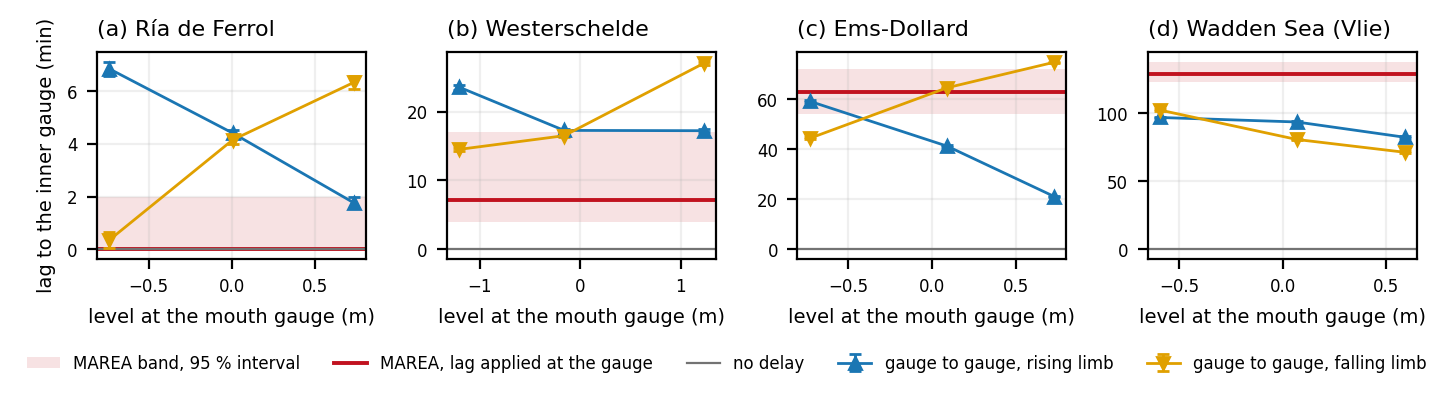
\includegraphics[width=\textwidth]{fig_lag_external.png}
\caption{The interior lag against the gauge pairs. Lag between the mouth
gauge and the inner gauge in reaching the same level, 2023--2025, at the
25th, 50th and 75th percentile of the mouth's level, rising and falling
limb (mean over paired cycles, bars: standard error); the lag MAREA
applies at the inner gauge (line) with the 95\,\% bootstrap interval of
its band (shading); no delay at zero.}
\label{fig:lag_external}
\end{figure*}

\begin{figure*}[!tbp]
\centering
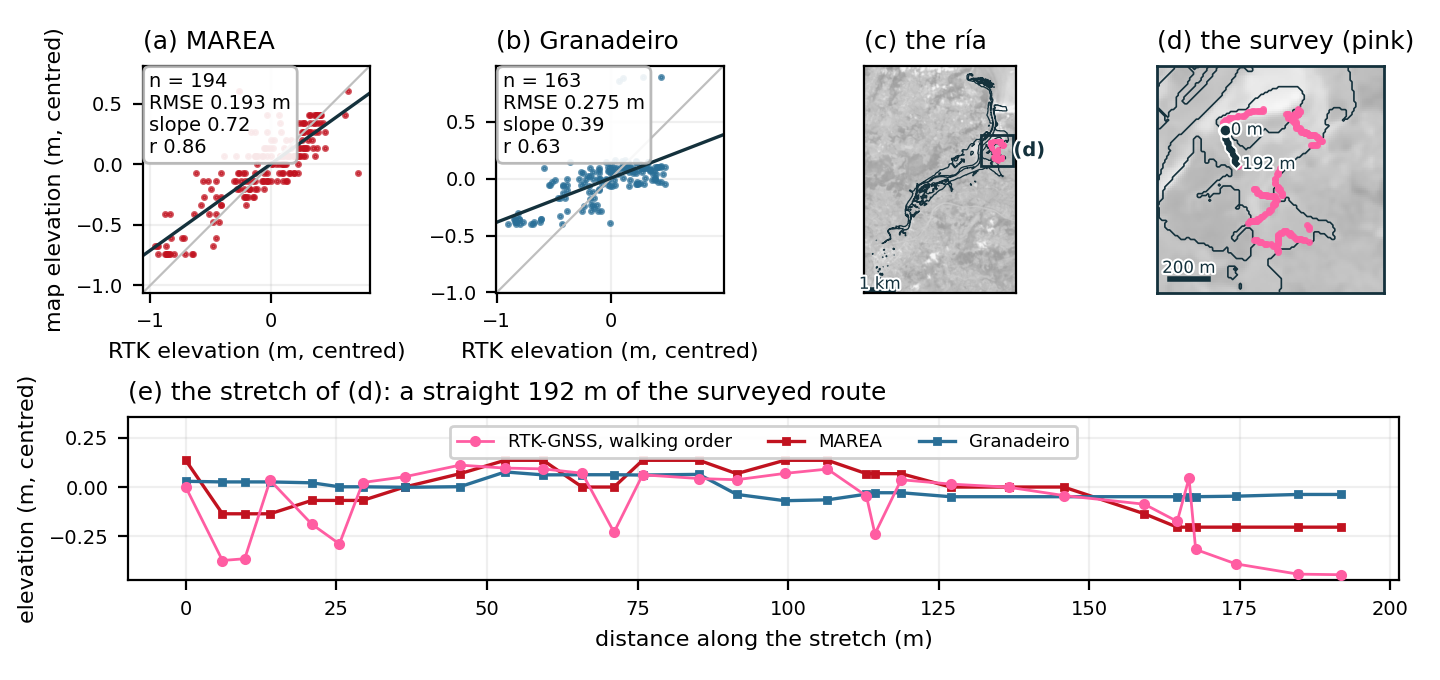
\includegraphics[width=\textwidth]{fig_rtk_onsite.png}
\caption{Elevation against the RTK-GNSS survey, Villaviciosa development
subset. (a), (b) Each map on the RTK elevation, both centred on their
medians, with the OLS line (dark) and the 1:1 line (grey). (c) The
R\'ia on the low-water scene, intertidal zone outlined, surveyed points
in pink; (d) the survey, with the straight stretch of (e) in white and
its start at 0~m. (e) Profile along that stretch: the RTK points joined
in walking order and the two maps at the pixels the route crosses, each
series centred.}
\label{fig:rtk_onsite}
\end{figure*}

\begin{figure*}[!tbp]
\centering
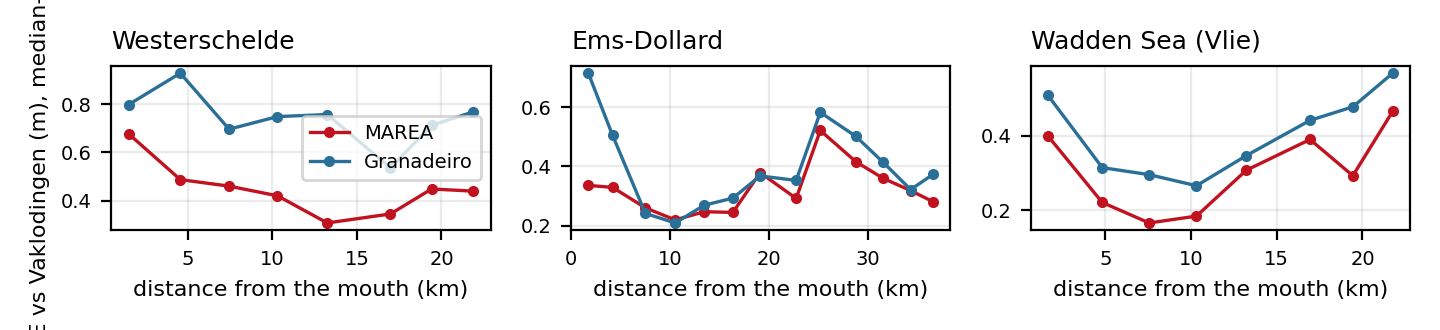
\includegraphics[width=\textwidth]{fig_vaklodingen_bands.png}
\caption{RMSE against the Vaklodingen by band of distance from the mouth,
median-centred, for the two maps at the three Dutch sites.}
\label{fig:vaklodingen_bands}
\end{figure*}

\end{document}
